\documentclass[dvips,landscape]{foils}
\usepackage{graphicx}
\usepackage{graphics}
\usepackage{amsmath}
\usepackage{amsthm}
\usepackage[all]{xy}
\usepackage{amsfonts}
\input defs.tex
\raggedright
\special{! TeXDict begin /landplus90{true}store end }
\renewcommand{\oursection}[1]{
\foilhead[-1.0cm]{#1}
}

\graphicspath{{figures/}}

\title{Cutoffs in Chaotic Map Mixing and Topology Optimization of Microfluidic Channels}
\author{Tzu-Chen Liang}
\MyLogo{Tzu-Chen Liang, Stanford University}
\date{\today}
\newtheorem{definition}{Definition}
\newtheorem{example}{Example}
\newtheorem{theorem}{Theorem}
\newtheorem{lemma}{Lemma}
\DeclareMathOperator{\erf}{erf}
\DeclareMathOperator{\prob}{\mathbf{Prob}}


% Here are the 3 topics
\newcommand{\mytopica}{Topology Optimization of Microfluidic Channels}
\newcommand{\mytopicb}{Numerical Evidence of Cutoffs in Chaotic Mixing}
\newcommand{\mytopicc}{Symbolic Dynamics and Cutoff Phenomenon}


\begin{document}
%\setlength{\parskip}{0cm}
\maketitle
%%%%%%%%%%%%%%%%%%%%%%%%%%%%%%%%%%%%%%%%%%%%%%%%%%%%%%%%%%%%%%%%%%%%%%%%
\newpage
\oursection{Outline}
\begin{itemize}
\item \mytopica
\item \mytopicb
\item \mytopicc
\end{itemize}
%%%%%%%%%%%%%%%%%%%%%%%%%%%%%%%%%%%%%%%%%%%%%%%%%%%%%%%%%%%%%%%%%%%%%%%%%
%%%%%%%%%%%%%%%%%%%%%%%%%%%%%%%%%%%%%%%%%%%%%%%%%%%%%%%%%%%%%%%%%%%%%%%%%
%%%%%%%%%%%%%                 TOPIC a                          %%%%%%%%%%
%%%%%%%%%%%%%%%%%%%%%%%%%%%%%%%%%%%%%%%%%%%%%%%%%%%%%%%%%%%%%%%%%%%%%%%%%
%%%%%%%%%%%%%%%%%%%%%%%%%%%%%%%%%%%%%%%%%%%%%%%%%%%%%%%%%%%%%%%%%%%%%%%%%
\newpage
\oursection{\mytopica}
   \begin{itemize}
      \item Microfluidics and the Mixing Problem
      \item Forming the optimization problem
     % \item Finding a decent direction
      \item Methods and Tools 
      \item Results
      \item How chaotic mixing works?
   \end{itemize}


%%%%%%%%%%%%%%%%%%%%%%%%%%%%%%%%%%%%%%%%%%%%%%%%%%%%%%%%%%%%%%%%%%%%%%%%%
%%%%%%%%%%%%%%%%%%%%%%%%%%%%%%%%%%%%%%%%%%%%%%%%%%%%%%%%%%%%%%%%%%%%%%%%%
\newpage
\oursection{Microfluidics and the Mixing Problem}
%%%%%%%%%%%%%%%%%%%%%%%%%%%%%%%%%%%%%%%%%%%%%%%%%%%%%%%%%%%%%%%%%%%%%%%%%
%\vspace{-1.5cm} 
%  \begin{itemize}\setlength{\parskip}{0pt}  \setlength{\itemsep}{5pt} \setlength{\topsep}{0pt}
%  \item Water in channel with cross-section $\ell \approx 100\,\mu\text{m}$.
%  \item Reynolds number $\text{Re} = U\ell/\nu < 100$.
%  \item P\'eclet number $\text{Pe} = U\ell/D \approx 10^6$.
%  \item Required channel length $\gg 10\,\text{cm}$, growing linearly with $\text{Pe}$.
%  \item Chaotic mixing protocol is suggested, and believed to have the best mixing. 
%  \end{itemize}
 
%  \begin{center}
%      \centerline{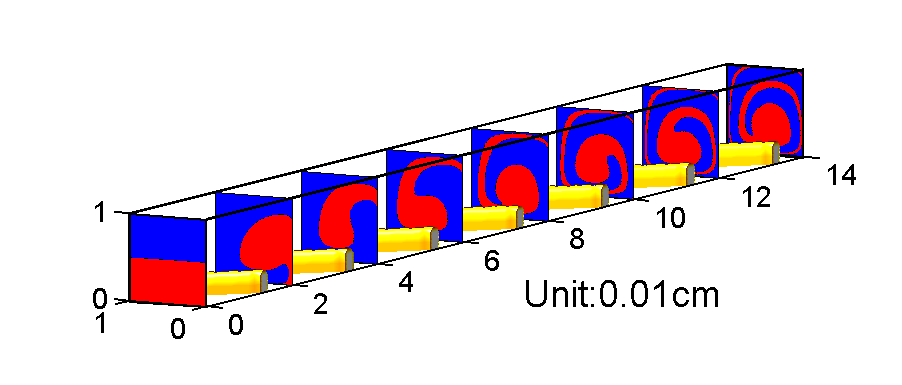
\includegraphics[width=0.5\textwidth,trim=1cm 0.5cm 1cm 0cm]{mixingchannel}}
%  \end{center}
 
\begin{itemize}
\item Microfluidic systems control and manipulate liquids in microliter or nanoliter scale.
\item Microfluidic mixing channel: objective is to mix two different liquids thoroughly.
\item Reynolds number $\text{Re} = \frac{Ul}{\nu}\approx 1$: flow is laminar.  P\'{e}clet number $\text{Pe} = \frac{Ul}{D} \gg 1$: diffusion is slow comparing with convection.
\item For example: $\text{Pe}=10^5$, the length of a smooth channel required for mixing is $10^3\,\text{cm}$. It grows linearly with $\text{Pe}$.
\item Chaotic mixing protocols is suggested in the design of mixing channel, and believed to have the best mixing.
\end{itemize}


%%%%%%%%%%%%%%%%%%%%%%%%%%%%%%%%%%%%%%%%%%%%%%%%%%%%%%%%%%%%%%%%%%%%%%%%%
\newpage
\oursection{\bfseries Stroock's Staggered Herringbone Mixer}
%%%%%%%%%%%%%%%%%%%%%%%%%%%%%%%%%%%%%%%%%%%%%%%%%%%%%%%%%%%%%%%%%%%%%%%%%
%%%%%%%%%%%%%%%%%%%%%%%%%%%%%%%%%%%%%%%%%%%%%%%%%%%%%%%%%%%%%%%%%%%%%%%%%
  \begin{figure}
    \centerline{
       \scalebox{0.3}[0.3]{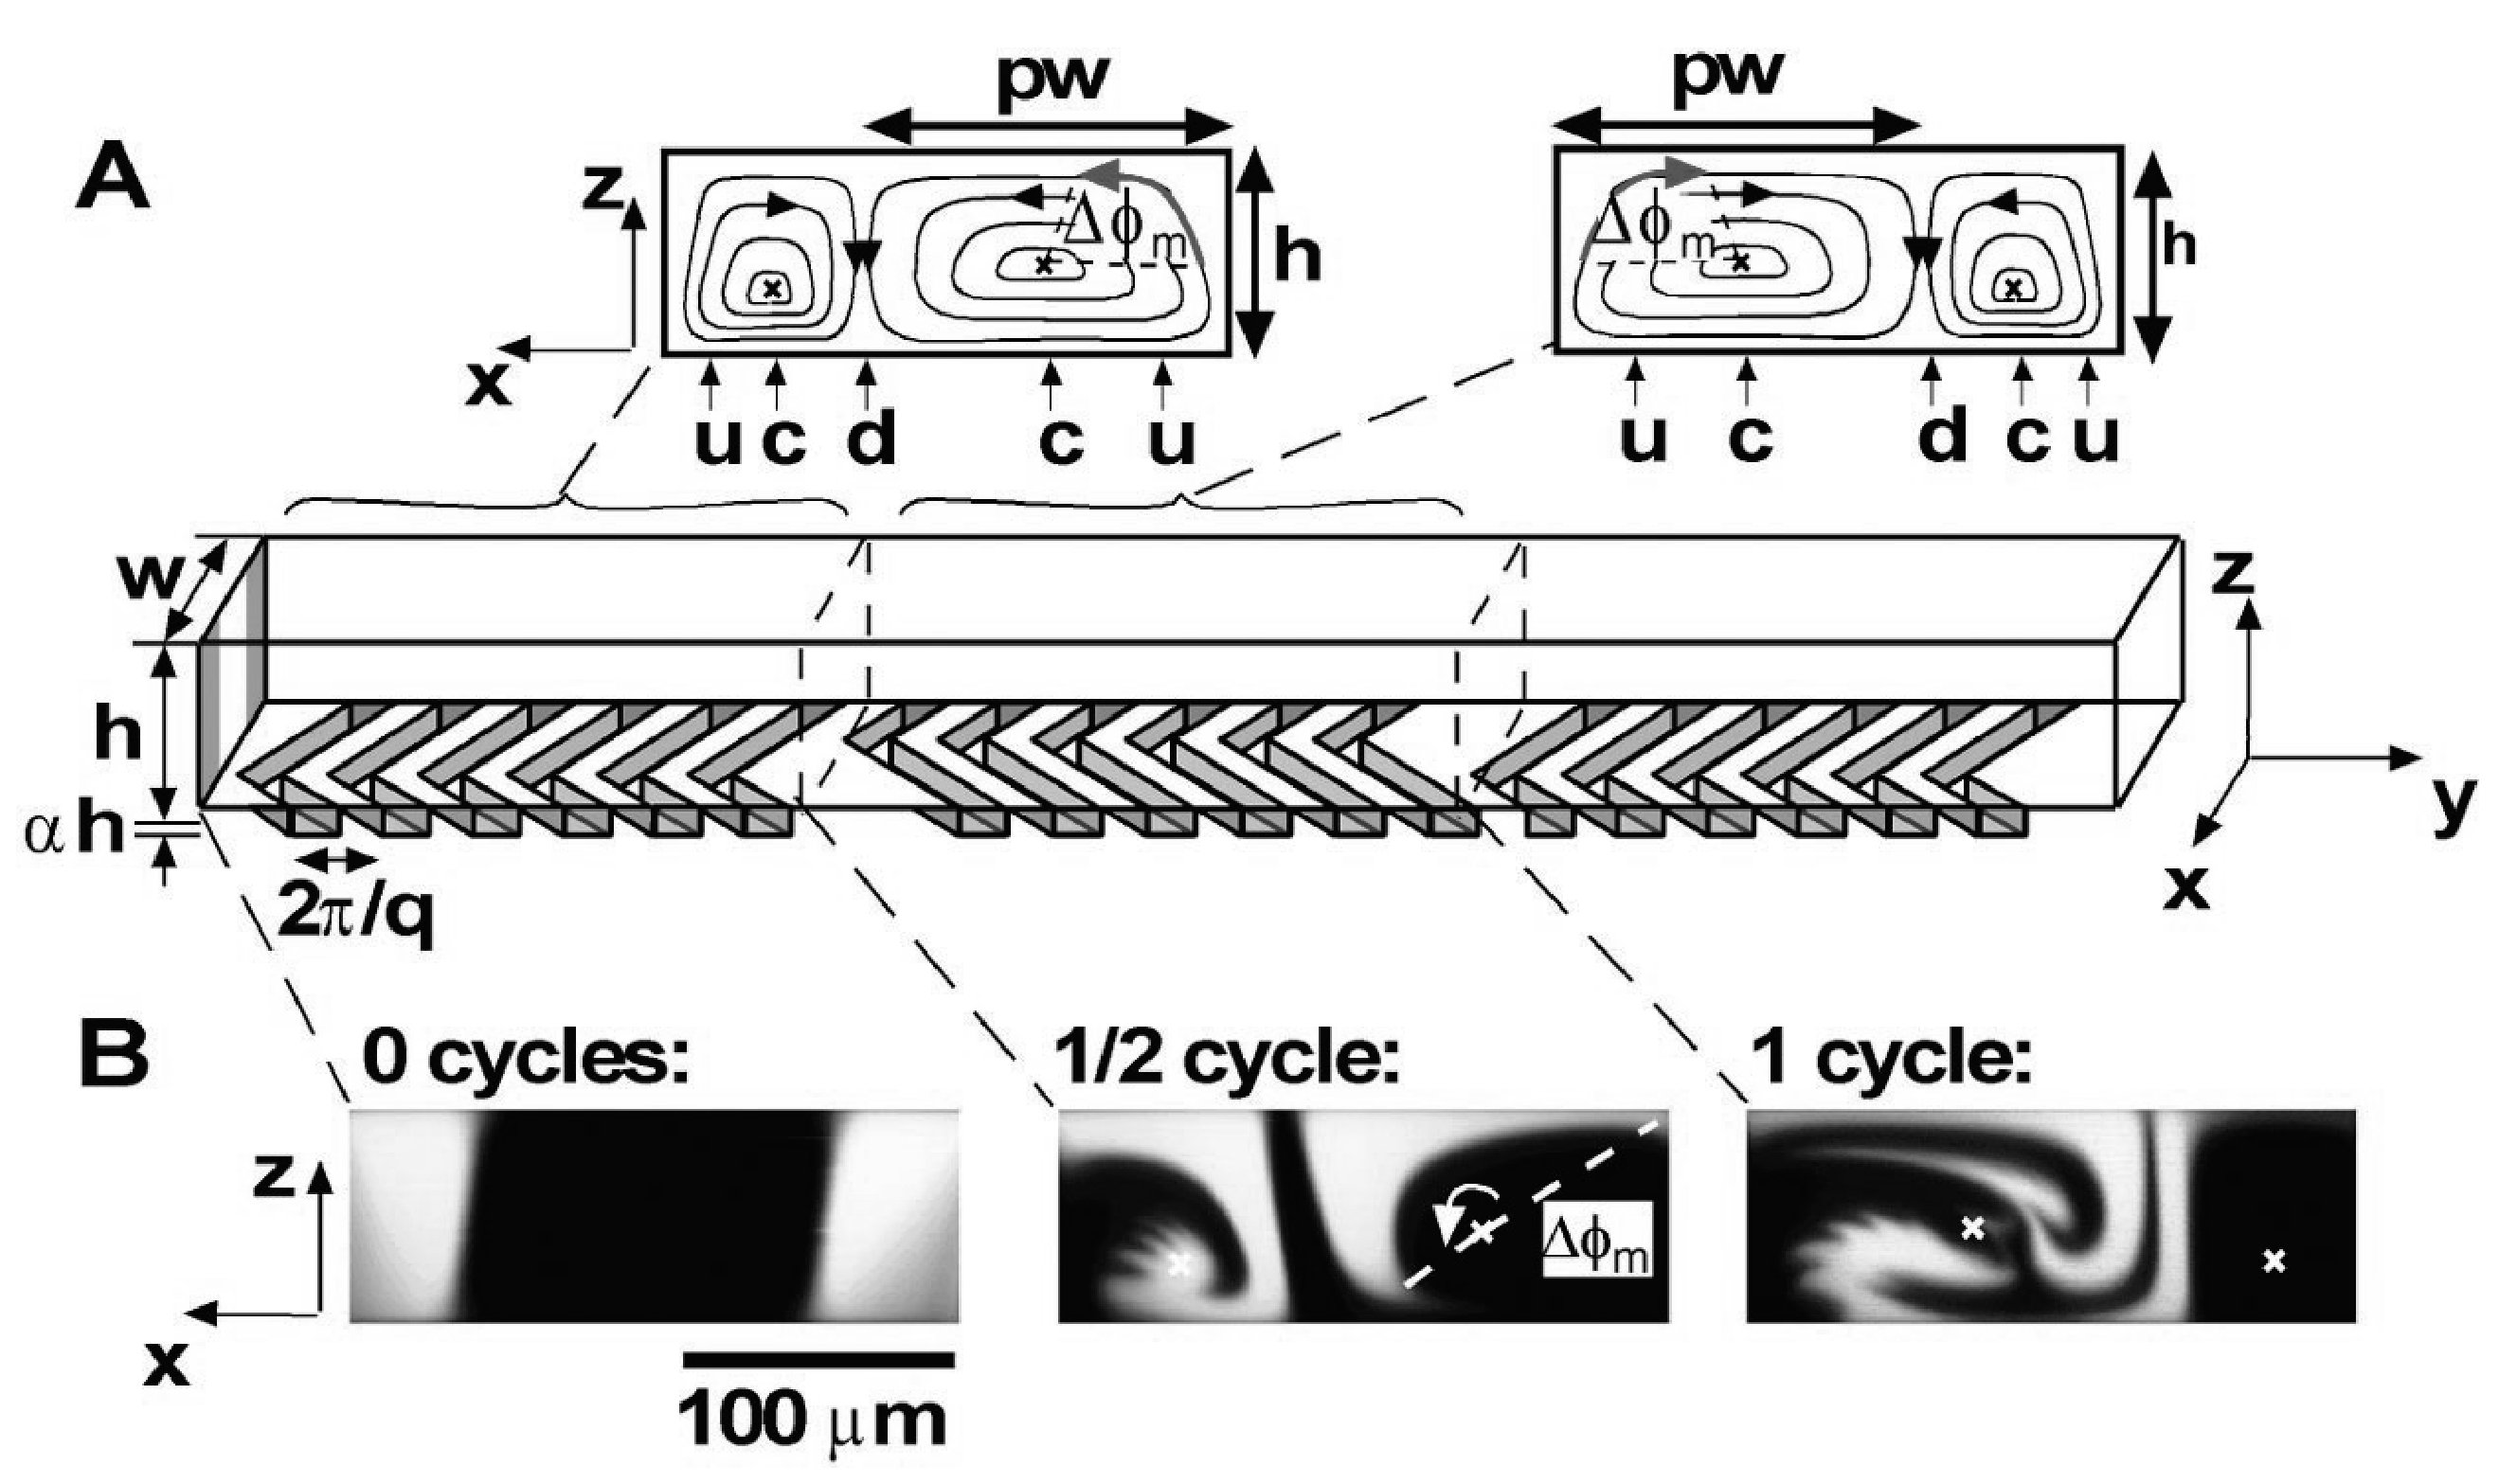
\includegraphics{stroockmixer}}
       \scalebox{0.6}[0.6]{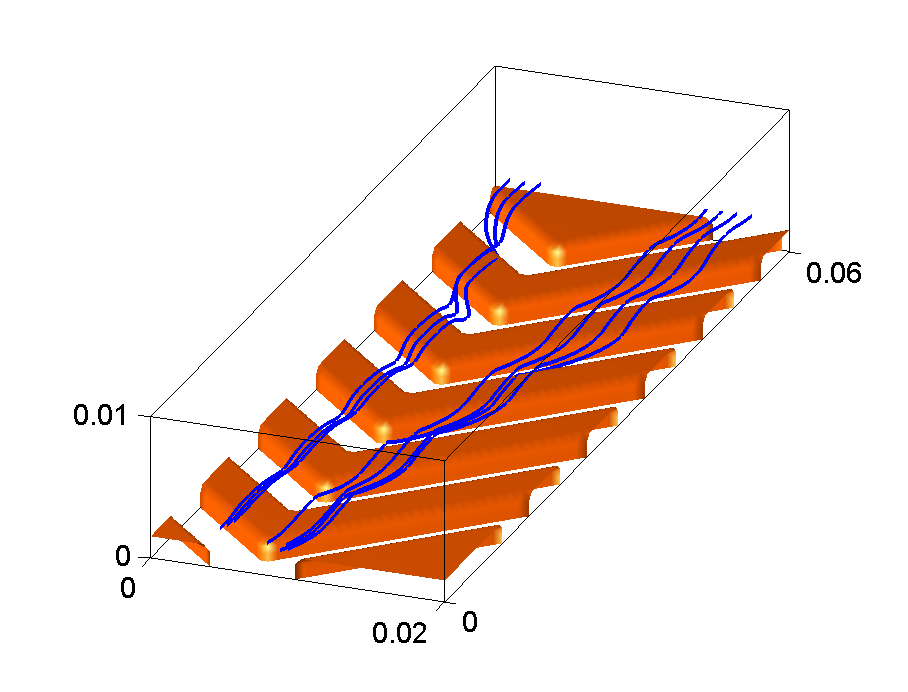
\includegraphics{stroockstructure}}
    }
  \end{figure}
\vspace{-1cm}
\begin{itemize}\setlength{\parskip}{0pt}  \setlength{\itemsep}{10pt} \setlength{\topsep}{0pt}
\item Stroock, Dertinger, Ajdari, Mezi\'c, Stone, Whitesides, \textit{Science} \textbf{295} (2002).  
\item Mixing length grows linearly with $\log(\text{Pe})$. 
\item Our Goal: improve it by applying topology optimization on the half-cycle structure. 
\end{itemize}



%%%%%%%%%%%%%%%%%%%%%%%%%%%%%%%%%%%%%%%%%%%%%%%%%%%%%%%%%%%%%%%%%%%%%%%%%
%%%%%%%%%%%%%%%%%%%%%%%%%%%%%%%%%%%%%%%%%%%%%%%%%%%%%%%%%%%%%%%%%%%%%%%%%
\newpage
\oursection{Topology Optimization}
\begin{itemize}
  \item A typical topology optimization problem is to distribute a given amount of material in a design domain subject to load and support conditions such that the stiffness of the structure is maximized.
  \item No initial knowledge about the structure.
  \item When applying to the mixing channel design,
  \begin{itemize}\setlength{\parskip}{0pt}  \setlength{\itemsep}{5pt} \setlength{\topsep}{0pt}
    \item A large problem ($144\times 24\times 72$ fluid/structure grids: over $10^6$ variables.)
    \item Nonlinear(nonconvex) optimization.
    %\item No clear defined measure of mixing.
    %\item No clear way to realize the Linked Twist Map (LTM) design procedure.
  \end{itemize}
\end{itemize}

%%%%%%%%%%%%%%%%%%%%%%%%%%%%%%%%%%%%%%%%%%%%%%%%%%%%%%%%%%%%%%%%%%%%%%%%%
%%%%%%%%%%%%%%%%%%%%%%%%%%%%%%%%%%%%%%%%%%%%%%%%%%%%%%%%%%%%%%%%%%%%%%%%%
\newpage
\oursection{Stokes Equation, Darcey Flow and Objective Functions}

\begin{itemize}\setlength{\parskip}{0pt}  \setlength{\itemsep}{5pt} \setlength{\topsep}{0pt}
\item Generalized Stokes partial differential equation for imcompressible flow (Darcey equation)
       \begin{eqnarray*}
         \begin{aligned}
       ( -\nu\Delta + \alpha ) u +\nabla  p & = f\\
       \text{div} u& =  0
         \end{aligned}
       \end{eqnarray*}
       
       $u$: velocity, $p$: pressure, $f$: body force and boundary conditions
       $\nu$: kinematic viscosity, and $\alpha$: inverse permeability

\item Objective functions
  \begin{itemize}
      \item $g(u)=c^T u$: As a heuristic we maximize downward velocity between the two vortices.
  %    \item Can differentiate particle streamlines with respect to $u$ and
  %    $\alpha$, allowing objective functions involving the particle map.  
  \end{itemize}




%\item Discrete version
%       \begin{equation}
%       \left[\begin{matrix}
%       -\nu \mathbf{L} + \mathbf{H} \mathbf{\bar{\alpha}}  & \mathbf{G}\\
%       \mathbf{D}               &  0
%       \end{matrix} \right]
%    \left[\begin{matrix}
%    \mathbf{\bar{u}} \\ \mathbf{\bar{p}}
%    \end{matrix} \right]=
%    \left[\begin{matrix}
%    \mathbf{\bar{f}} \\ \mathbf{0}
%    \end{matrix} \right]
%    \end{equation}

\end{itemize}

%%%%%%%%%%%%%%%%%%%%%%%%%%%%%%%%%%%%%%%%%%%%%%%%%%%%%%%%%%%%%%%%%%%%%%%%%
%%%%%%%%%%%%%%%%%%%%%%%%%%%%%%%%%%%%%%%%%%%%%%%%%%%%%%%%%%%%%%%%%%%%%%%%%
\newpage
\oursection{Forming the optimization problem}
Topology optimization problem:
\begin{align*}
      \text{minimize } & g(u,p,\alpha) \\
      \text{subject to } & \begin{bmatrix} -\nu L + \alpha H & G \\
        D & 0 \end{bmatrix} \begin{bmatrix} u \\ p \end{bmatrix}
      = \begin{bmatrix} f \\ 0 \end{bmatrix} \\
      & 0 \le \alpha \le \alpha_{\text{max}}\\
\intertext{Lump the equality constraints into the objective function:}
     \text{minimize } & g(u(\alpha),p(\alpha),\alpha) \\
   \text{subject to } &  0 \le \alpha \le \alpha_{\text{max}}
\end{align*}


%%%%%%%%%%%%%%%%%%%%%%%%%%%%%%%%%%%%%%%%%%%%%%%%%%%%%%%%%%%%%%%%%%%%%%%%%
%%%%%%%%%%%%%%%%%%%%%%%%%%%%%%%%%%%%%%%%%%%%%%%%%%%%%%%%%%%%%%%%%%%%%%%%%
\newpage
\oursection{Methods and Tools}
%%%%%%%%%%%%%%%%%%%%%%%%%%%%%%%%%%%%%%%%%%%%%%%%%%%%%%%%%%%%%%%%%%%%%%%%%
Methods
\vspace{-0.8cm}
\begin{itemize}\setlength{\parskip}{0pt}  \setlength{\itemsep}{10pt} \setlength{\topsep}{0pt}
\item Finite difference method with staggered mesh to solve the flow field.
\item Adjoint method to find $\frac{dg}{d\alpha}$ without forming $\frac{du}{d\alpha}$.
\item A gradient-based optimization scheme with fixed step size.
\item A \textbf{Markov Chain} model to approximate the solution of the advection-diffusion equation on the cross-sections of the channel.
\item Fourth order Runge-Kutta method to integrate streamlines.
\end{itemize}
\vspace{-0.6cm}
Tools
\vspace{-0.8cm}
\begin{itemize}\setlength{\parskip}{0pt}  \setlength{\itemsep}{10pt} \setlength{\topsep}{0pt}
\item PETSc(Portable, Extensible Toolkit for Scientific Computation)
%\item Develope a package that communicates PETSc and Matlab
\item A 72-node PC cluster. 1G bytes memory for each CPU and gigabytes intranet connection.
\end{itemize}


%%%%%%%%%%%%%%%%%%%%%%%%%%%%%%%%%%%%%%%%%%%%%%%%%%%%%%%%%%%%%%%%%%%%%%%%%
\newpage
\oursection{Optimal 2D and 3D Structures}
%%%%%%%%%%%%%%%%%%%%%%%%%%%%%%%%%%%%%%%%%%%%%%%%%%%%%%%%%%%%%%%%%%%%%%%%%
%%%%%%%%%%%%%%%%%%%%%%%%%%%%%%%%%%%%%%%%%%%%%%%%%%%%%%%%%%%%%%%%%%%%%%%%%
%\begin{example}
  \begin{figure}
    \centerline{
       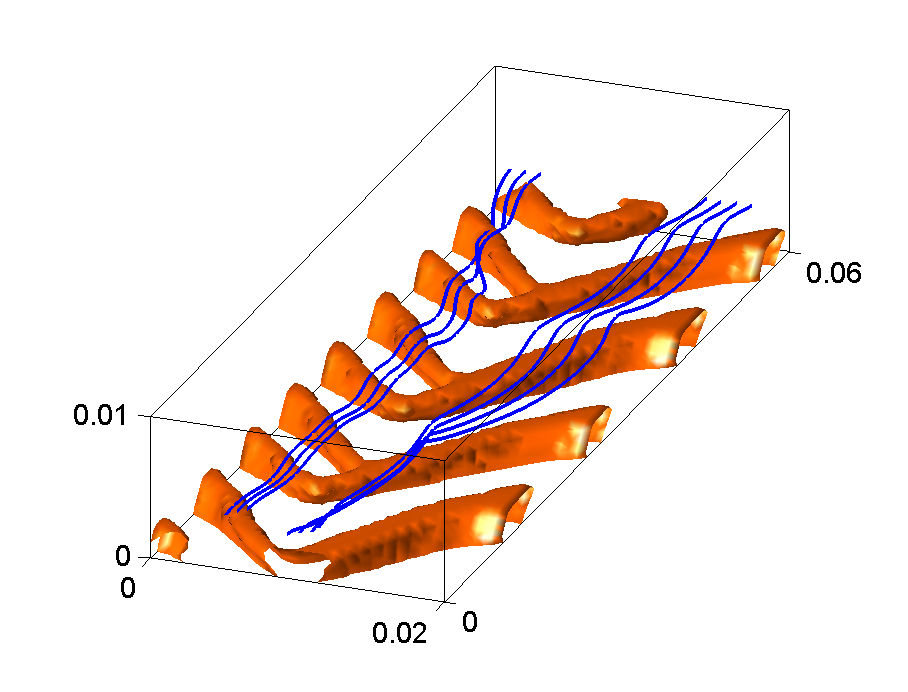
\includegraphics[width=0.45\textwidth,trim=1cm 0cm 0cm 0cm,clip]{myharringbonestructure}
       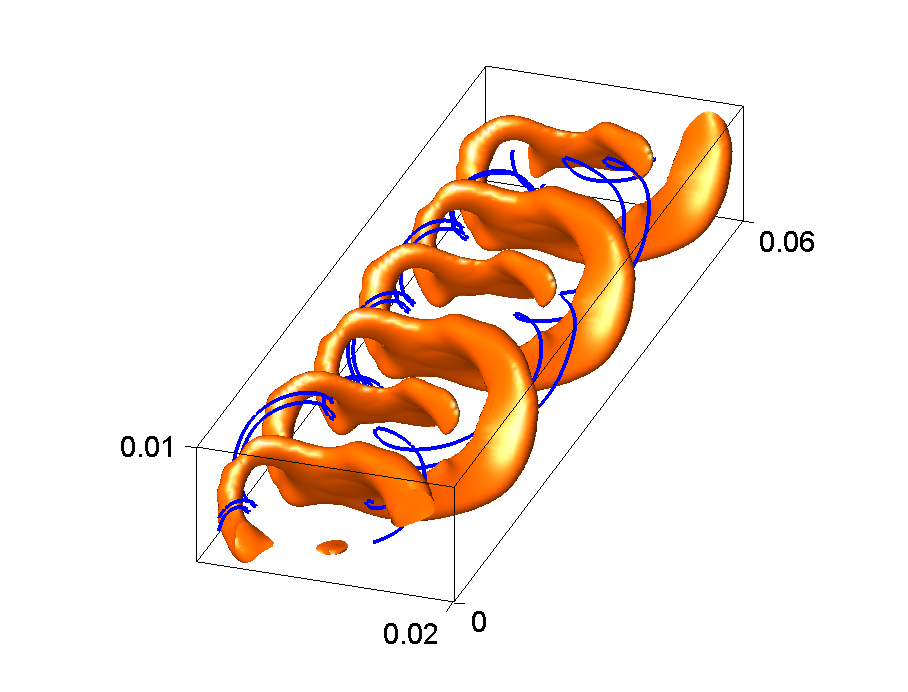
\includegraphics[width=0.45\textwidth,trim=1cm 0cm 1cm 0cm,clip]{my3dstructure}     
    }
  \end{figure}
\begin{itemize}\setlength{\parskip}{0pt}  \setlength{\itemsep}{10pt} \setlength{\topsep}{0pt}
\item Left: Optimal herringbone channel.
\item Right: Optimal 3-D structured channel.  
\end{itemize}

%%%%%%%%%%%%%%%%%%%%%%%%%%%%%%%%%%%%%%%%%%%%%%%%%%%%%%%%%%%%%%%%%%%%%%%%%
%%%%%%%%%%%%%%%%%%%%%%%%%%%%%%%%%%%%%%%%%%%%%%%%%%%%%%%%%%%%%%%%%%%%%%%%%
\newpage
\oursection{Build a Full Cycle}
%%%%%%%%%%%%%%%%%%%%%%%%%%%%%%%%%%%%%%%%%%%%%%%%%%%%%%%%%%%%%%%%%%%%%%%%%
%  \begin{figure}
%    \centerline{
%       \scalebox{0.65}[0.65]{\includegraphics{mixersimu}}
%       \scalebox{0.65}[0.65]{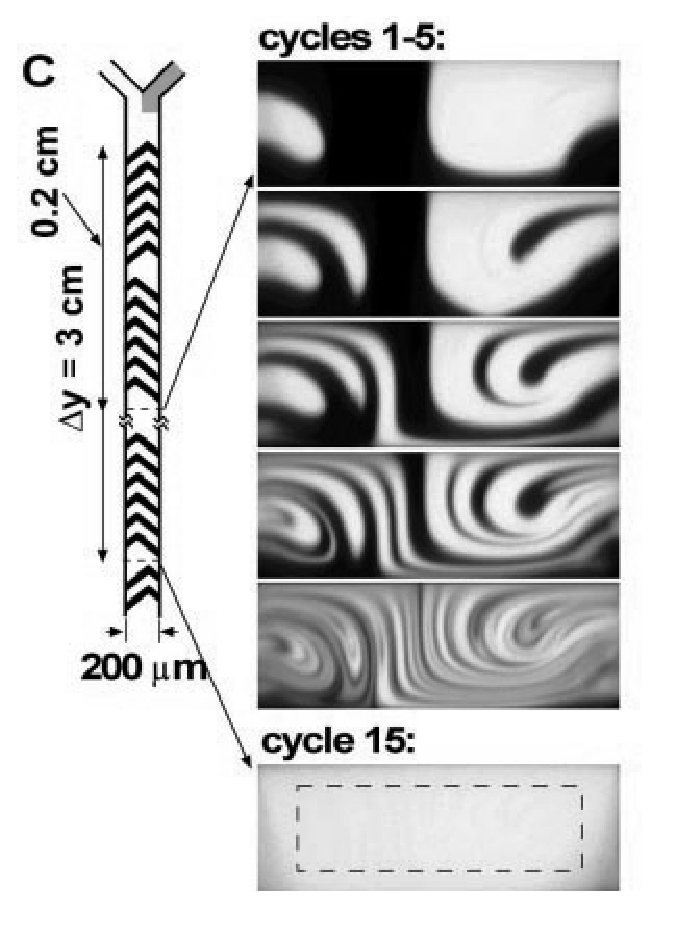
\includegraphics{stroockcrosssection0}}
%    }
%  \end{figure}
%\vspace{-0.5cm}
%\begin{figure}  
%       \scalebox{0.60}[0.60]{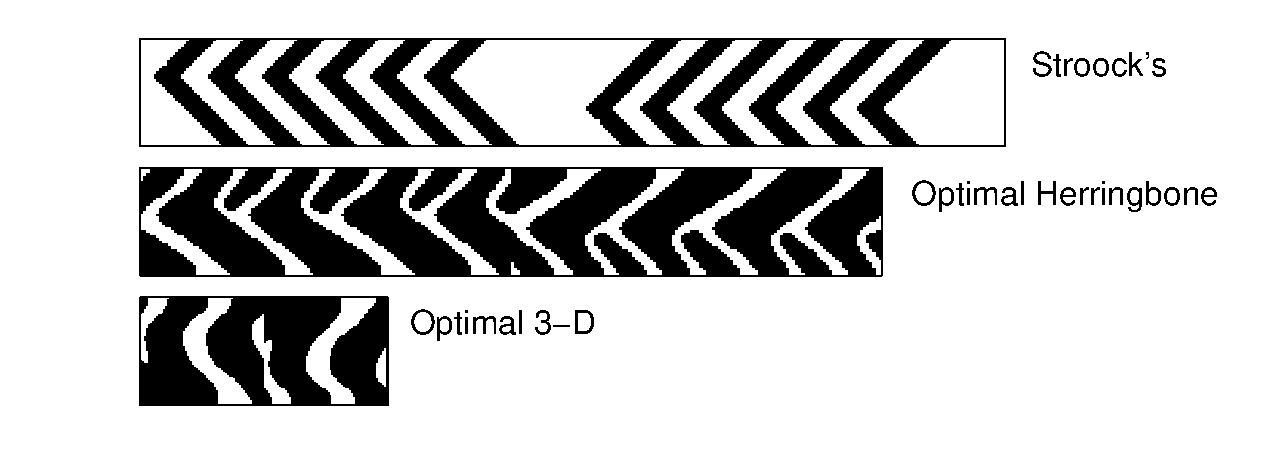
\includegraphics[trim=-2cm 0cm 0cm 0cm,clip]{example2fullcycle}}
%\end{figure}  
\begin{itemize}
\item A full cycle of mixing channel is composed of two half-cycle channels. 
\item We try different number of periodical structures per half-cycle to find the best combination.   
\end{itemize}
\begin{figure}  
       \scalebox{0.9}[0.9]{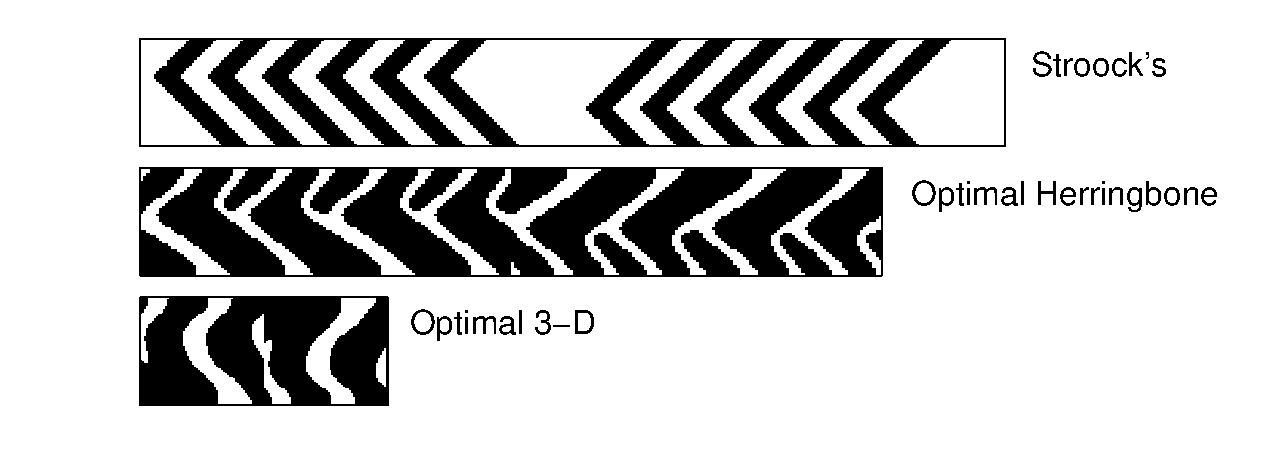
\includegraphics[trim=-2cm 0cm 0cm 0cm,clip]{example2fullcycle}}
\end{figure}  

%%%%%%%%%%%%%%%%%%%%%%%%%%%%%%%%%%%%%%%%%%%%%%%%%%%%%%%%%%%%%%%%%%%%%%%%%
%%%%%%%%%%%%%%%%%%%%%%%%%%%%%%%%%%%%%%%%%%%%%%%%%%%%%%%%%%%%%%%%%%%%%%%%%
\newpage
\oursection{Mixing Length}
%%%%%%%%%%%%%%%%%%%%%%%%%%%%%%%%%%%%%%%%%%%%%%%%%%%%%%%%%%%%%%%%%%%%%%%%%

  \begin{figure}
    \centerline{
       \scalebox{0.6}[0.6]{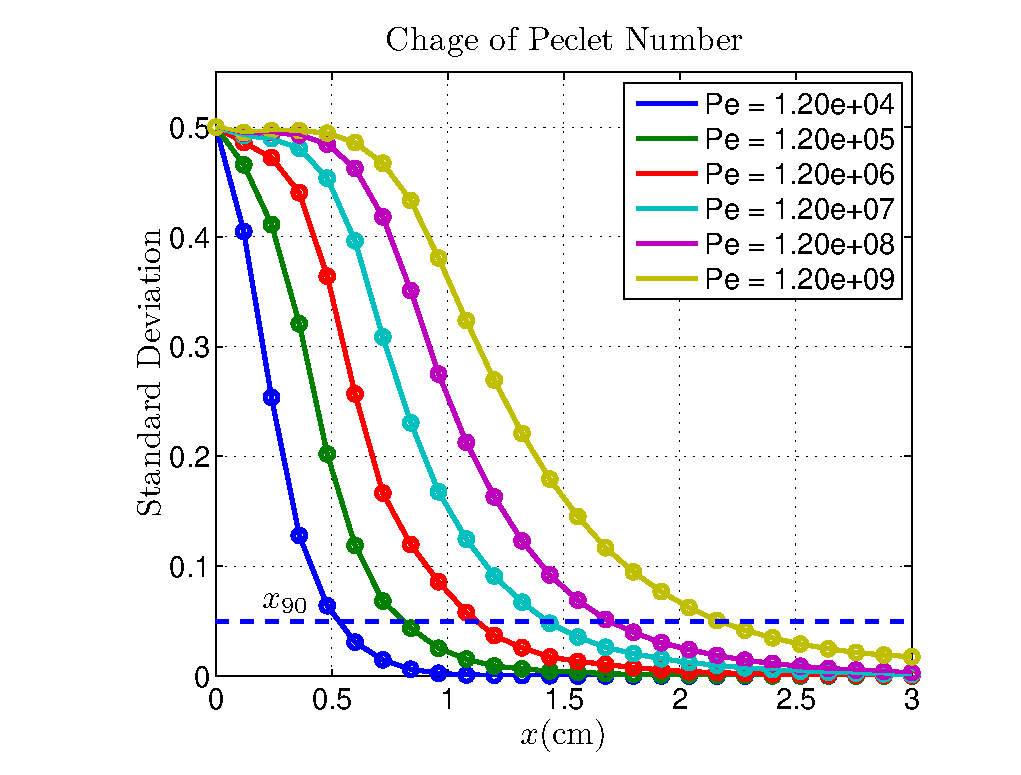
\includegraphics{example2veryPe2}}
       \scalebox{0.6}[0.6]{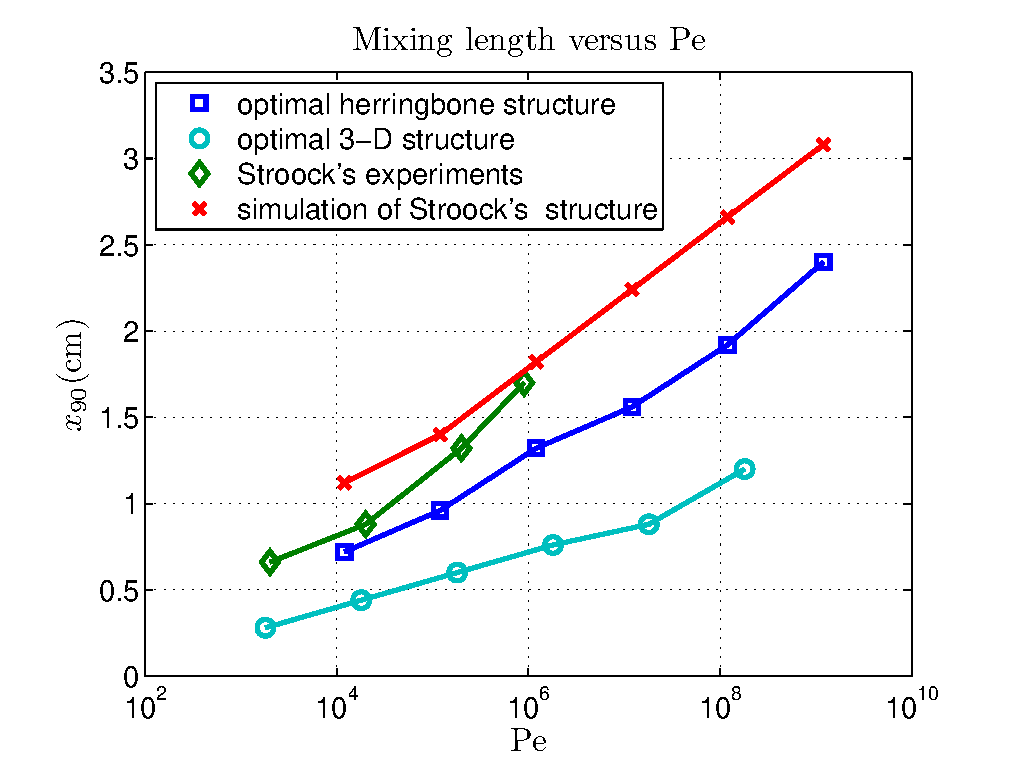
\includegraphics{example2mixinglength2}}
    }
  \end{figure}
%\end{example}
\begin{itemize}\setlength{\parskip}{0pt}  \setlength{\itemsep}{10pt} \setlength{\topsep}{0pt}
\item Mixing Length($x_{90}$) grows linearly with $\log(\text{Pe})$.
\item Optimal herringbone structure improves mixing length by 30\%,
    optimal 3D structure by 60\%.
\end{itemize}


%%%%%%%%%%%%%%%%%%%%%%%%%%%%%%%%%%%%%%%%%%%%%%%%%%%%%%%%%%%%%%%%%%%%%%%%%
\newpage
\oursection{More about Mixing: How Chaotic Mixing Works?}
%%%%%%%%%%%%%%%%%%%%%%%%%%%%%%%%%%%%%%%%%%%%%%%%%%%%%%%%%%%%%%%%%%%%%%%%%
%%%%%%%%%%%%%%%%%%%%%%%%%%%%%%%%%%%%%%%%%%%%%%%%%%%%%%%%%%%%%%%%%%%%%%%%%
\vspace{-0.5cm}
  \begin{figure}
    \centerline{
       \scalebox{0.70}[0.70]{\includegraphics{chaoticmixing}}
    }
  \end{figure}
\vspace{-0.3cm}
Three-stage transition on the variance trajectory.  
%%%%%%%%%%%%%%%%%%%%%%%%%%%%%%%%%%%%%%%%%%%%%%%%%%%%%%%%%%%%%%%%%%%%%%%%%
%%%%%%%%%%%%%%%%%%%%%%%%%%%%%%%%%%%%%%%%%%%%%%%%%%%%%%%%%%%%%%%%%%%%%%%%%
%\newpage
%\oursection{More about Mixing}
%%%%%%%%%%%%%%%%%%%%%%%%%%%%%%%%%%%%%%%%%%%%%%%%%%%%%%%%%%%%%%%%%%%%%%%%%
  %\begin{itemize}
  %\item Why not optimize mixing directly?
  %  \begin{itemize}
  %  \item Can't compute the gradient of mixing length.
  %  \end{itemize}
  %\item A question about the mixing trajectory.
  %\end{itemize}
  %\begin{center}
  %  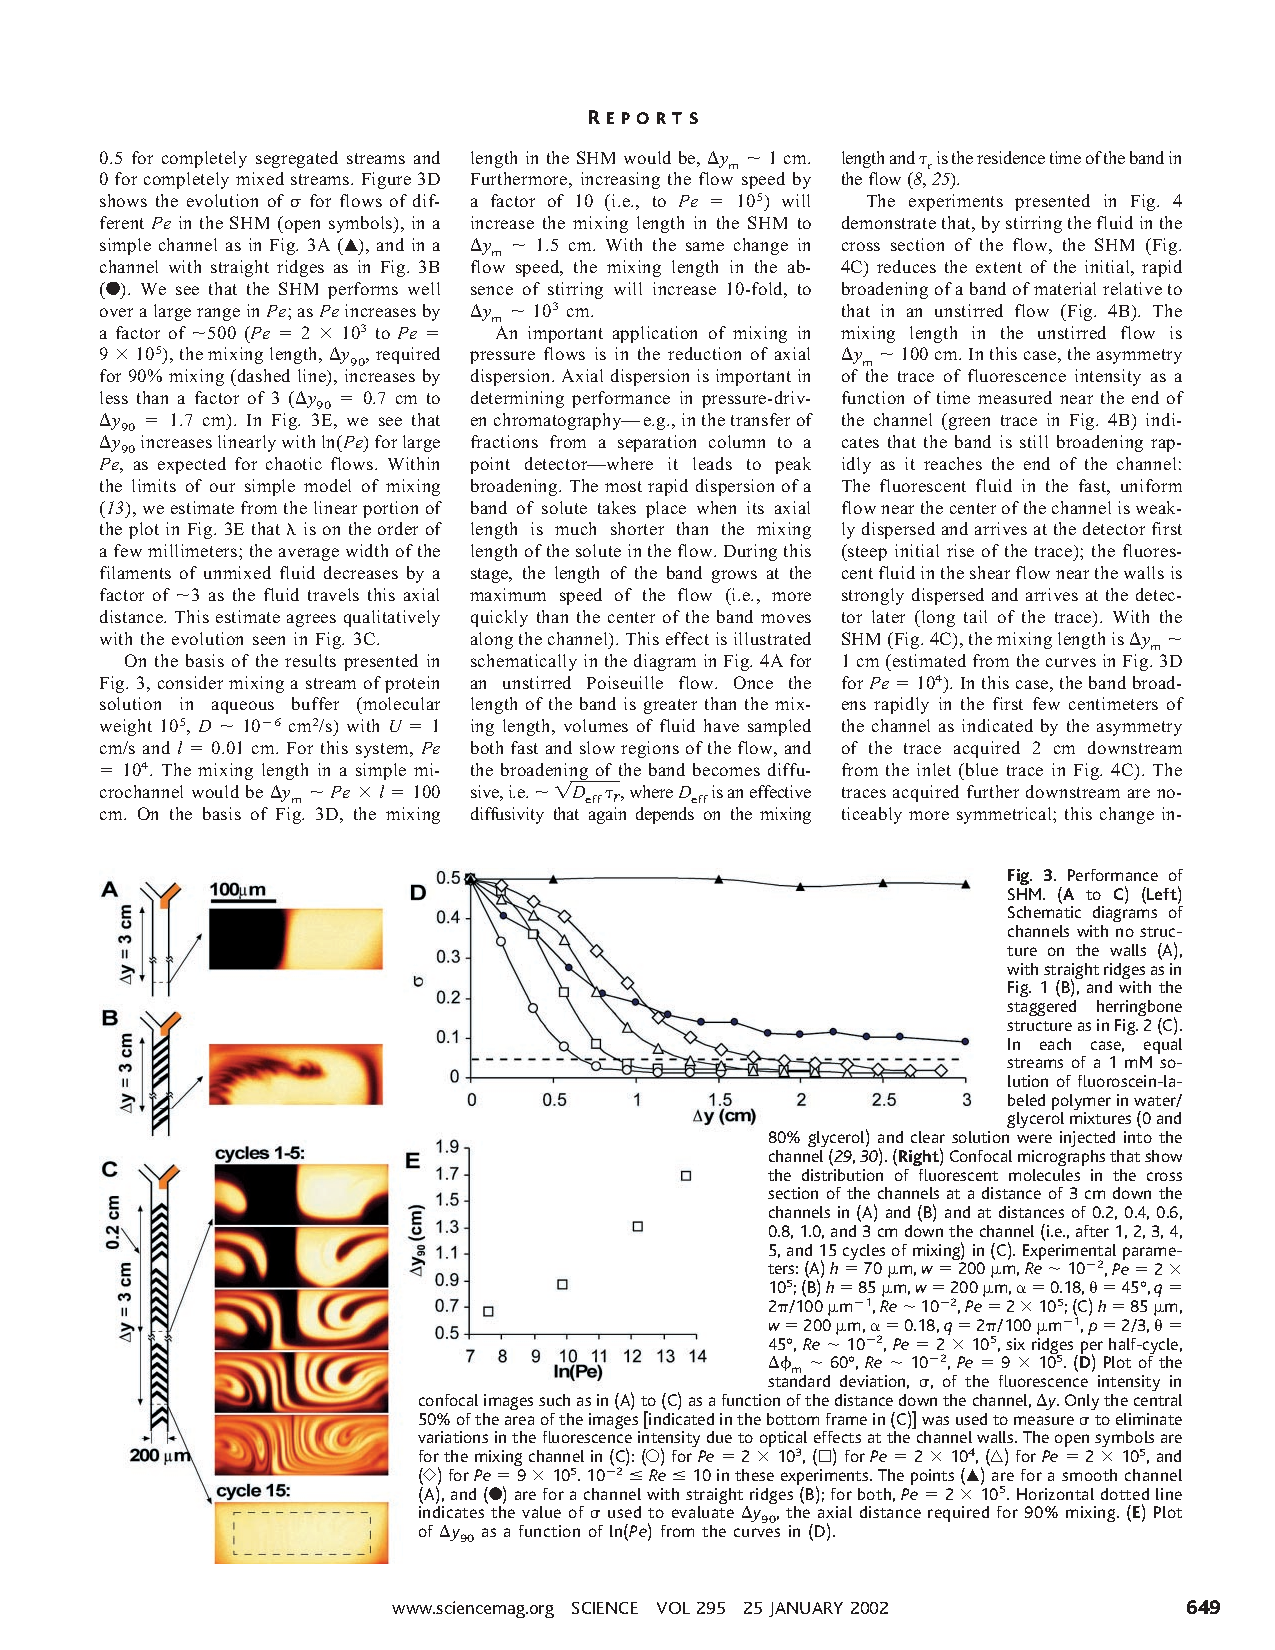
\includegraphics[height=4cm,trim=6.5cm 8.8cm 5cm 14cm,clip=true]{stroock_page3}
  %\end{center}



%%%%%%%%%%%%%%%%%%%%%%%%%%%%%%%%%%%%%%%%%%%%%%%%%%%%%%%%%%%%%%%%%%%%%%%%%
%%%%%%%%%%%%%%%%%%%%%%%%%%%%%%%%%%%%%%%%%%%%%%%%%%%%%%%%%%%%%%%%%%%%%%%%%
%%%%%%%%%%%%%                 TOPIC b                          %%%%%%%%%%
%%%%%%%%%%%%%%%%%%%%%%%%%%%%%%%%%%%%%%%%%%%%%%%%%%%%%%%%%%%%%%%%%%%%%%%%%
%%%%%%%%%%%%%%%%%%%%%%%%%%%%%%%%%%%%%%%%%%%%%%%%%%%%%%%%%%%%%%%%%%%%%%%%%

%%%%%%%%%%%%%%%%%%%%%%%%%%%%%%%%%%%%%%%%%%%%%%%%%%%%%%%%%%%%%%%%%%%%%%%%%
%%%%%%%%%%%%%%%%%%%%%%%%%%%%%%%%%%%%%%%%%%%%%%%%%%%%%%%%%%%%%%%%%%%%%%%%%
\newpage
\oursection{\mytopicb}
%%%%%%%%%%%%%%%%%%%%%%%%%%%%%%%%%%%%%%%%%%%%%%%%%%%%%%%%%%%%%%%%%%%%%%%%%
\begin{itemize}\setlength{\parskip}{0pt}  \setlength{\itemsep}{5pt} \setlength{\topsep}{0pt}
  \item How the variance changes when a scalar function is evolved by a chaotic map and the diffusion goes to zero.
  \item Bringing cutoff phenomenon from finite Markov Chain studies to chaotic map mixing.
  \item Numerical evidence of Standard map cutoffs.
\end{itemize}
Why Standard map?
\vspace{-0.5cm}
\begin{itemize}\setlength{\parskip}{0pt}  \setlength{\itemsep}{5pt} \setlength{\topsep}{0pt}
\item Most researches are focused on the property of the map itself, not the Perron-Frobenius or Koopman operators of it.
\item Known numerical results have poor resolution($500 \times 500$).
  We use up to $80000\times 80000$ number of grids. $51.2$ Gbytes of memory is required. %to store a single state vector.
\item The issue of numerical diffusion versus physical diffusion.
\end{itemize}

%%%%%%%%%%%%%%%%%%%%%%%%%%%%%%%%%%%%%%%%%%%%%%%%%%%%%%%%%%%%%%%%%%%%%%%%%
%%%%%%%%%%%%%%%%%%%%%%%%%%%%%%%%%%%%%%%%%%%%%%%%%%%%%%%%%%%%%%%%%%%%%%%%%
\newpage
\oursection{Cutoff Phenomenon}
%%%%%%%%%%%%%%%%%%%%%%%%%%%%%%%%%%%%%%%%%%%%%%%%%%%%%%%%%%%%%%%%%%%%%%%%%
\begin{example} \textbf{Random walk on an $n$-dimensional hypercube}
a particle starts at $\mathbf{0}$ and moves to one of its nearest neighbors (or stay fixed) with equal probability at each step.

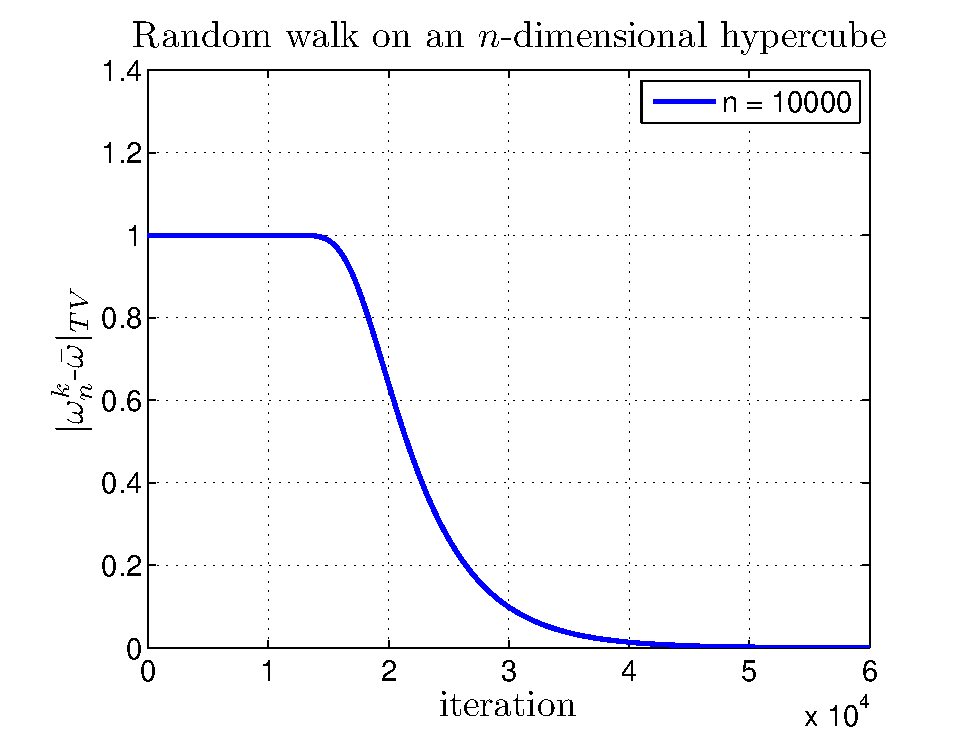
\includegraphics[width=0.45\textwidth,trim=1cm 1cm 0cm 0cm]{rdwalk1}
\parbox[b]{12cm}{
 \begin{itemize}\setlength{\parskip}{0pt}  \setlength{\itemsep}{5pt} \setlength{\topsep}{0pt}
  \item A Markov Chain with $2^n$ states.
  \item The invariant distribution $\bar{\omega}_n$ is uniform. 
  \item $|\omega^k_n - \bar{\omega}_n|_{TV}$, where $k$ is the number of iterations. 
 \end{itemize}
  \textbf{Total Variation Distance}
  \begin{eqnarray*}
   |\mu - \nu|_{TV} = \frac{1}{2}\sum_{i=1}^n |\mu(i)-\nu(i) |
  \\[-2cm]
  \end{eqnarray*}
   }

\end{example} 
%%%%%%%%%%%%%%%%%%%%%%%%%%%%%%%%%%%%%%%%%%%%%%%%%%%%%%%%%%%%%%%%%%%%%%%%%
%%%%%%%%%%%%%%%%%%%%%%%%%%%%%%%%%%%%%%%%%%%%%%%%%%%%%%%%%%%%%%%%%%%%%%%%%
\newpage
\oursection{Cutoff in Finite Markov Chains}
%%%%%%%%%%%%%%%%%%%%%%%%%%%%%%%%%%%%%%%%%%%%%%%%%%%%%%%%%%%%%%%%%%%%%%%%%
  \begin{itemize}\setlength{\parskip}{0pt}  \setlength{\itemsep}{5pt} \setlength{\topsep}{0pt}
  \item Finite set $\Omega$ with ``metric'' $D$ on
    probability measures $\mu$, $\nu$, so that
    $D(\mu,\nu)$ such that 
    \begin{enumerate}
    \item $D(\mu,\nu)\in [0,1]$
    \item $\max_{\Omega,\mu,\nu} D(\mu,\nu) = 1$
    \item $D(\mu,\nu)=0$ if and only if $\mu=\nu$
    \end{enumerate}
  \item Sequence of probability spaces $(\Omega_n, \bar{\omega}_n)$,
    $n=1,2,\ldots$, each with a sequence of probability measures
    $\omega^k_n$, $l=0,1,\ldots$, such that
    \begin{align*}
      \lim_{k \rightarrow \infty} D(\omega^k_n,\bar{\omega}_n)=0
      \\[-1.6cm]
    \end{align*}
  \item Think of $n$ as dimension of a Markov Chain, $k$ as iteration
    number, $\omega^0_n$ as initial distribution, $\bar{\omega}_n$ as invariant
    distribution.
  %\item Examples: riffle shuffle of $n$ cards, random walk on
  %  $n$-dimensional hypercube, Ehrenfest's urn with $n$ balls, \ldots
  \end{itemize}


%%%%%%%%%%%%%%%%%%%%%%%%%%%%%%%%%%%%%%%%%%%%%%%%%%%%%%%%%%%%%%%%%%%%%%%%%
%%%%%%%%%%%%%%%%%%%%%%%%%%%%%%%%%%%%%%%%%%%%%%%%%%%%%%%%%%%%%%%%%%%%%%%%%
\newpage
\oursection{Cutoff Phenomenon}
%%%%%%%%%%%%%%%%%%%%%%%%%%%%%%%%%%%%%%%%%%%%%%%%%%%%%%%%%%%%%%%%%%%%%%%%%
\begin{definition}
\label{cutoffdefinition} (Diaconis) A family $(\Omega_n,\bar{\omega}_n, (\omega^k_n)_{k=0,1,...})_{n=1,2,...}$ presents a D-cut-off if
there exists a sequence $(t_n)$ of positive reals such that, for any $\epsilon \in(0,1)$,
\vspace{-1cm}
\begin{enumerate}\setlength{\parskip}{0pt}  \setlength{\itemsep}{5pt} \setlength{\topsep}{0pt}
  \item $\lim_{n \rightarrow \infty}D(\omega^{k_n}_n,\bar{\omega}_n) = 0 \mbox{ if }
  k_n>(1+\epsilon)t_n$
  \item $\lim_{n \rightarrow \infty}D(\omega^{k_n}_n,\bar{\omega}_n) = 1 \mbox{ if }
  k_n<(1-\epsilon)t_n $
\end{enumerate}

\end{definition}
\centerline{
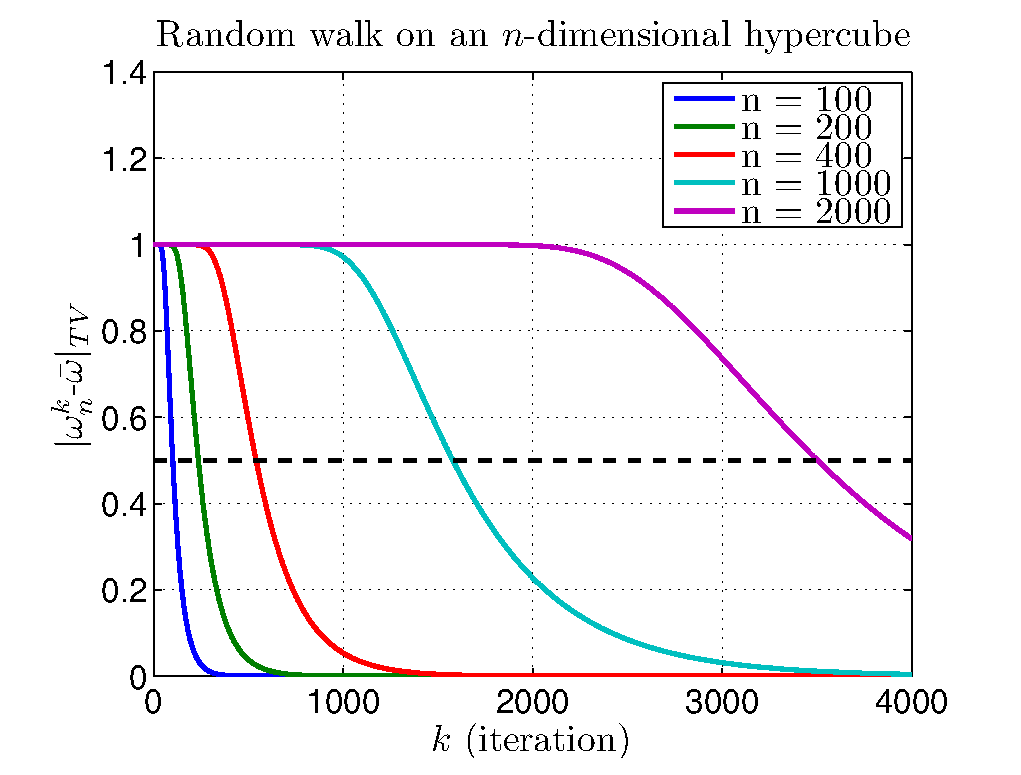
\includegraphics[width=0.43\textwidth,trim=1cm 1cm 0cm 0cm]{rdwalk}
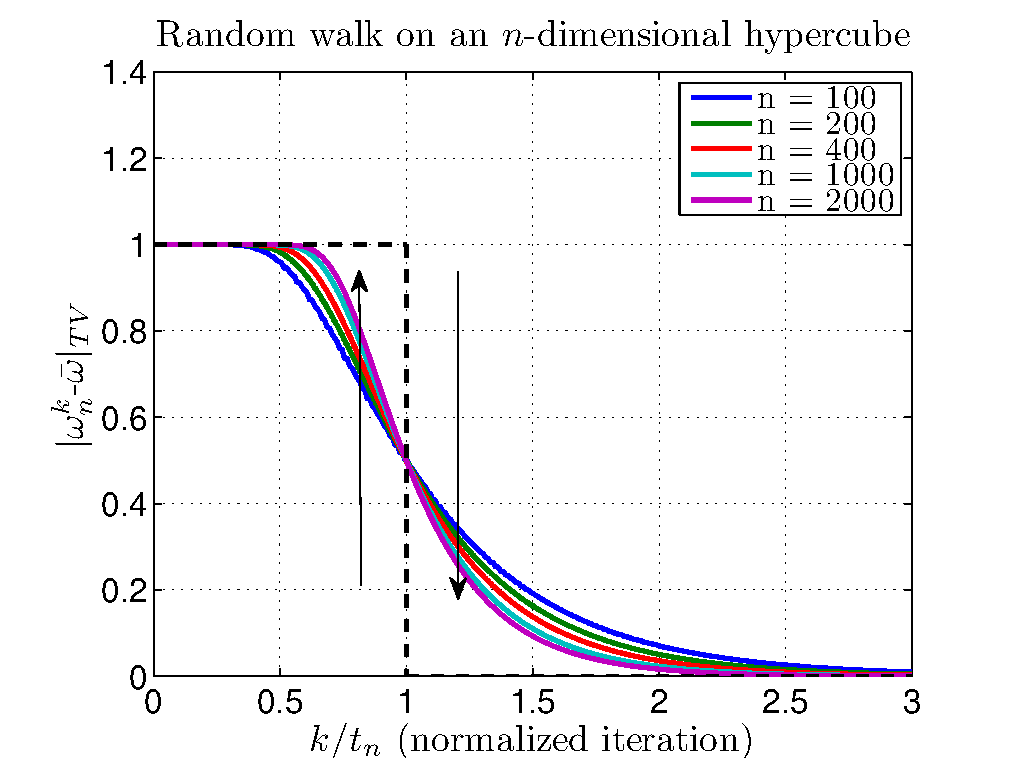
\includegraphics[width=0.43\textwidth,trim=1cm 1cm 0cm 0cm]{rdwalkn}
}



%%%%%%%%%%%%%%%%%%%%%%%%%%%%%%%%%%%%%%%%%%%%%%%%%%%%%%%%%%%%%%%%%%%%%%%%%
%%%%%%%%%%%%%%%%%%%%%%%%%%%%%%%%%%%%%%%%%%%%%%%%%%%%%%%%%%%%%%%%%%%%%%%%%
\newpage
\oursection{Perron-Frobenius Operator and Koopman Operator}
%%%%%%%%%%%%%%%%%%%%%%%%%%%%%%%%%%%%%%%%%%%%%%%%%%%%%%%%%%%%%%%%%%%%%%%%%
Given a map $S:X \rightarrow X$. In the measure space $(X,\mathcal{A},\mu)$,
\begin{definition} {\bfseries (Perron-Frobenius operator)}
Let $f \in L^1$, for every $A \in \mathcal{A}$ the operator $P:L^1 \rightarrow L^1$ satisfies
  \begin{eqnarray}
    \int_A Pf(x)\mu(dx) = \int_{S^{-1}(A)} f(x)\mu(dx)
  \end{eqnarray}
is the Perron-Frobenius operator associated with $S$.
\end{definition}


\begin{definition} {\bfseries (Koopman operator)}
Let $f \in L^\infty$. The operator $U:L^{\infty} \rightarrow L^{\infty} $ defined by
 \begin{eqnarray}
 Uf(x) = f(S(x))
 \end{eqnarray}
is called the Koopman operator associated with $S$.
\end{definition}
%%%%%%%%%%%%%%%%%%%%%%%%%%%%%%%%%%%%%%%%%%%%%%%%%%%%%%%%%%%%%%%%%%%%%%%%%
%%%%%%%%%%%%%%%%%%%%%%%%%%%%%%%%%%%%%%%%%%%%%%%%%%%%%%%%%%%%%%%%%%%%%%%%%
\newpage
\oursection{Scheme}
%%%%%%%%%%%%%%%%%%%%%%%%%%%%%%%%%%%%%%%%%%%%%%%%%%%%%%%%%%%%%%%%%%%%%%%%%
\begin{itemize}
\item Consider a discrete-time map $S:X\rightarrow X$.
\item Find either the Perron-Frobenius operator or the Koopman operator of $S$. 
\item The operator can be reduced by model reduction techniques. The result is a \textbf{Markov Chain}.
\item Diffusion can be added by a diffusion operator in spatial domain or in frequency domain.  \
\item This is also the strategy we use to approximate the solution of advection-diffusion equation of mixing channels.
\end{itemize}


%%%%%%%%%%%%%%%%%%%%%%%%%%%%%%%%%%%%%%%%%%%%%%%%%%%%%%%%%%%%%%%%%%%%%%%%%
\newpage
\oursection{Model Reduction}
%%%%%%%%%%%%%%%%%%%%%%%%%%%%%%%%%%%%%%%%%%%%%%%%%%%%%%%%%%%%%%%%%%%%%%%%%

\begin{tabular}{cl}
   \begin{tabular}{c}
      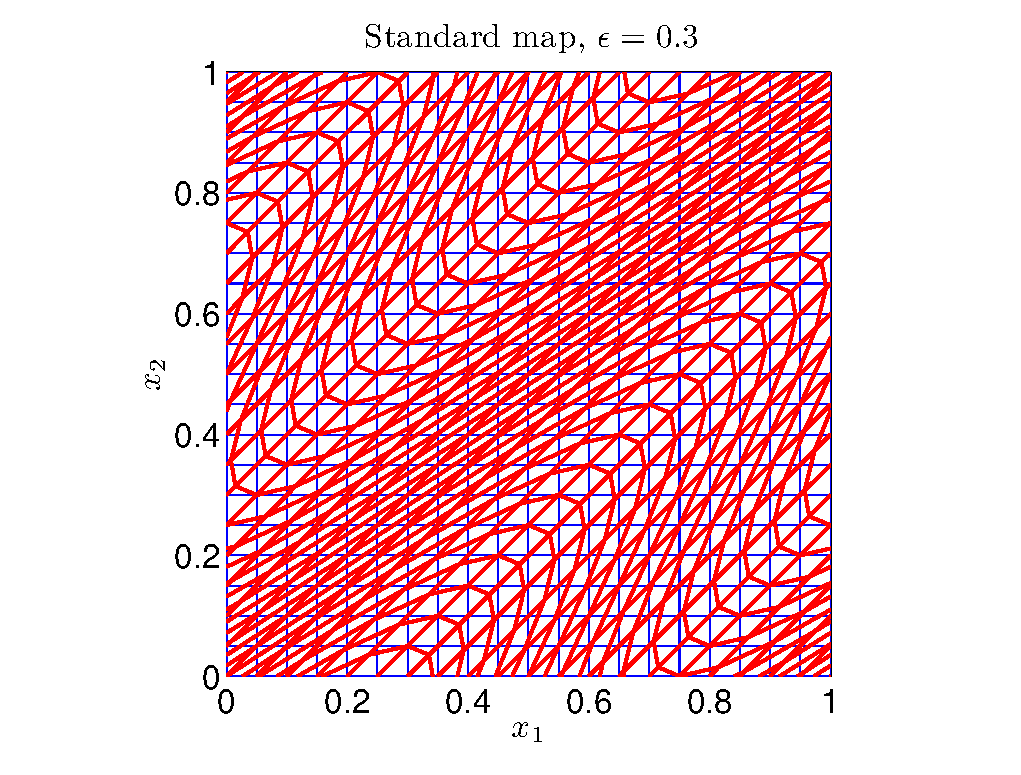
\includegraphics[width=0.45\textwidth,trim=2cm 1cm 2cm 1cm]{standardmapgrid}\\
      \begin{minipage}[s]{9cm}
   \vspace{0.4cm}

    \begin{eqnarray*}
       \text{Blue grids}:& a_i\\
       \text{Red  grids}:& S^{-1}(a_j)
    \end{eqnarray*}
      \end{minipage}
   \end{tabular}&
  \begin{minipage}[s]{10cm}
   \begin{itemize}\setlength{\parskip}{0pt}  \setlength{\itemsep}{5pt} \setlength{\topsep}{0pt}
    \item $X = [0,1] \times[0,1]$.
    \item $a_i, i=\{1,2,\cdots,n^2\}$ be regualr $n$ by $n$ grids on $X$.
    \item $\bar{\omega}$ is the invariant measure of $S$.
   \end{itemize}
  % The optimal model of Perron-Frobenius operator $A_n$ has 
   \begin{eqnarray*}
      \begin{aligned}
     (A_n)_{ij} & =  \text{Prob}(x^{k+1} \text{ in } a_j \mid x^{k} \text{ in }  a_i)  \\
                & = \frac{\bar{\omega}(S^{-1}(a_j)\cap a_i)}{\bar{\omega}(a_j)} 
      \end{aligned}
    \end{eqnarray*}
   \begin{itemize}\setlength{\parskip}{0pt}  \setlength{\itemsep}{5pt} \setlength{\topsep}{0pt}
   \item 
    \begin{eqnarray*}
     \begin{aligned}
      \\[-3cm]
        \omega_n^{k+1}& = A_n^T \omega_n^k\\ 
         f_n^{k}& = A_n f_n^{k+1} 
     \end{aligned}
     \end{eqnarray*}
   \end{itemize} 
   \end{minipage}
\end{tabular}


%   \begin{align}
%               x_1' &= x_1+x_2 \\%+\epsilon \sin{2 \pi x_1}  (\mbox{ mod } 1) \nonumber\\
%               x_2' &=  x_2 %+\epsilon \sin{2 \pi x_1}     (\mbox{ mod } 1)
%   \end{align}

%%%%%%%%%%%%%%%%%%%%%%%%%%%%%%%%%%%%%%%%%%%%%%%%%%%%%%%%%%%%%%%%%%%%%%%%%
%%%%%%%%%%%%%%%%%%%%%%%%%%%%%%%%%%%%%%%%%%%%%%%%%%%%%%%%%%%%%%%%%%%%%%%%%
\newpage
\oursection{Standard Map}
%%%%%%%%%%%%%%%%%%%%%%%%%%%%%%%%%%%%%%%%%%%%%%%%%%%%%%%%%%%%%%%%%%%%%%%%%
\vspace{-0.1cm}
\centerline{
\begin{tabular}{rl}%\setlength{\tabcolsep}{-30mm}
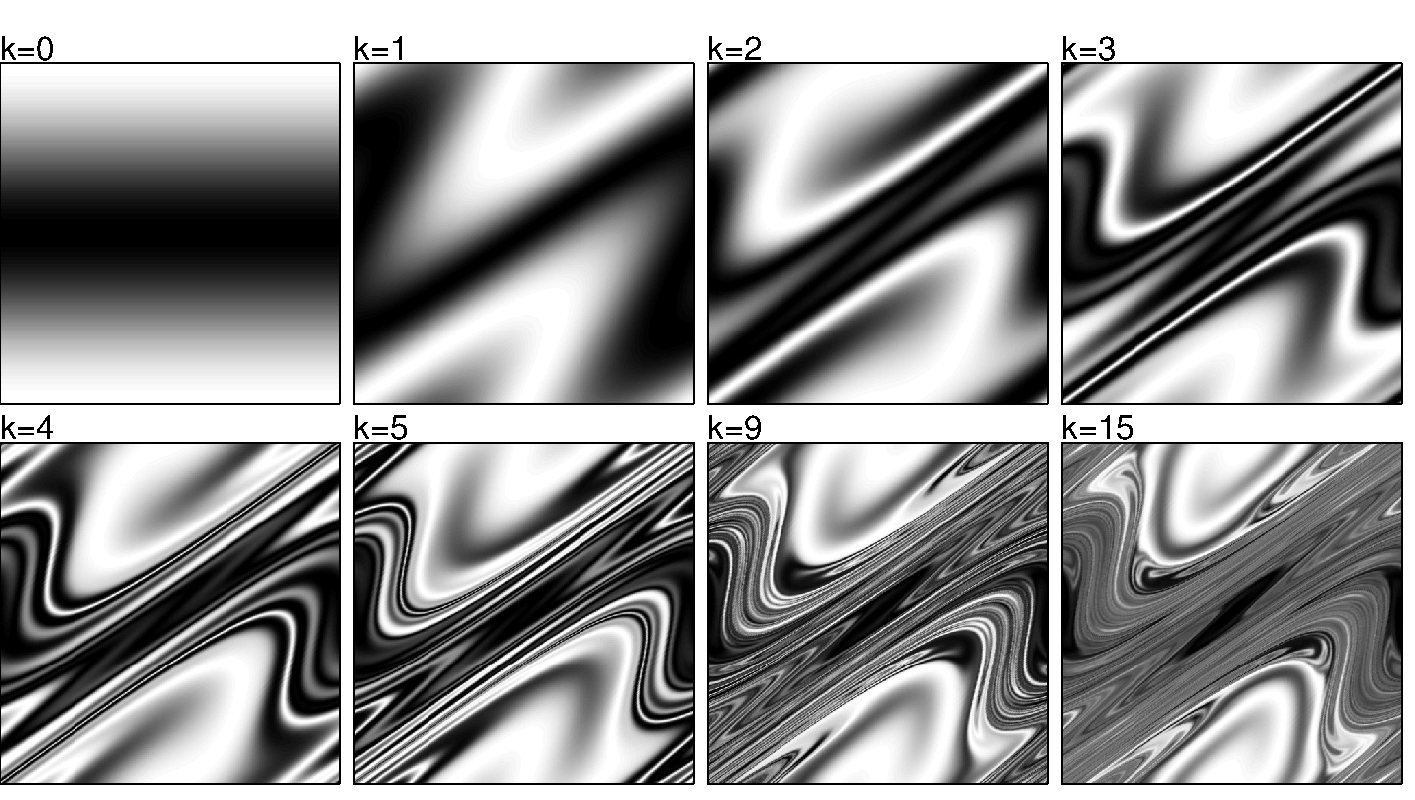
\includegraphics[width=0.75\textwidth,trim=1cm 1cm 0cm 0cm]{standardmapevolve}
%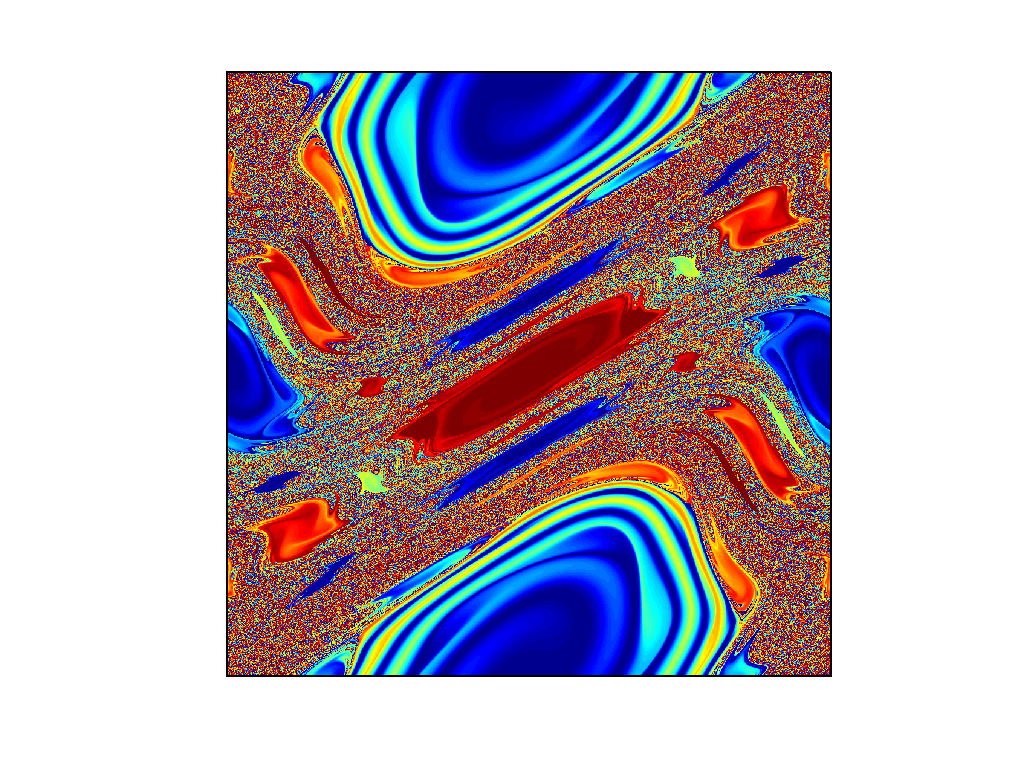
\includegraphics[width=0.52\textwidth,trim=1cm 1cm 0cm 0cm]{standardmapsimuexact}&
%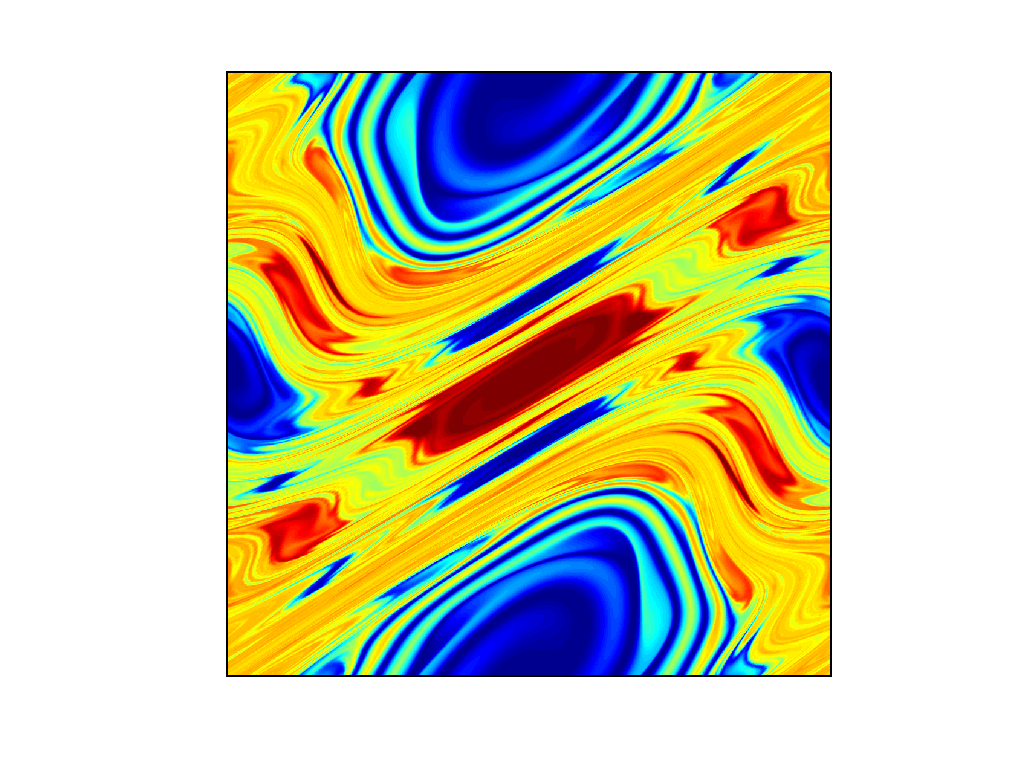
\includegraphics[width=0.52\textwidth,trim=1cm 1cm 0cm 0cm]{standardmapsimumarkov}
\end{tabular}
}
   \begin{equation*}
     \begin{cases}
        x_1 \leftarrow &x_1+x_2 +\epsilon \sin{2 \pi x_1}  (\mbox{ mod } 1)\\
        x_2 \leftarrow & x_2 +\epsilon \sin{2 \pi x_1}     (\mbox{ mod } 1) 
     \end{cases}     
   \end{equation*}
   \begin{equation*}
      \epsilon=0.3, \,\, f^0   = \cos(2\pi x_2)
   \end{equation*}



%%%%%%%%%%%%%%%%%%%%%%%%%%%%%%%%%%%%%%%%%%%%%%%%%%%%%%%%%%%%%%%%%%%%%%%%%
%%%%%%%%%%%%%%%%%%%%%%%%%%%%%%%%%%%%%%%%%%%%%%%%%%%%%%%%%%%%%%%%%%%%%%%%%
\newpage
\oursection{Evidence of Standard Map Cutoff}
%%%%%%%%%%%%%%%%%%%%%%%%%%%%%%%%%%%%%%%%%%%%%%%%%%%%%%%%%%%%%%%%%%%%%%%%%
\centerline{
\begin{tabular}{rl}%\setlength{\tabcolsep}{-30mm}
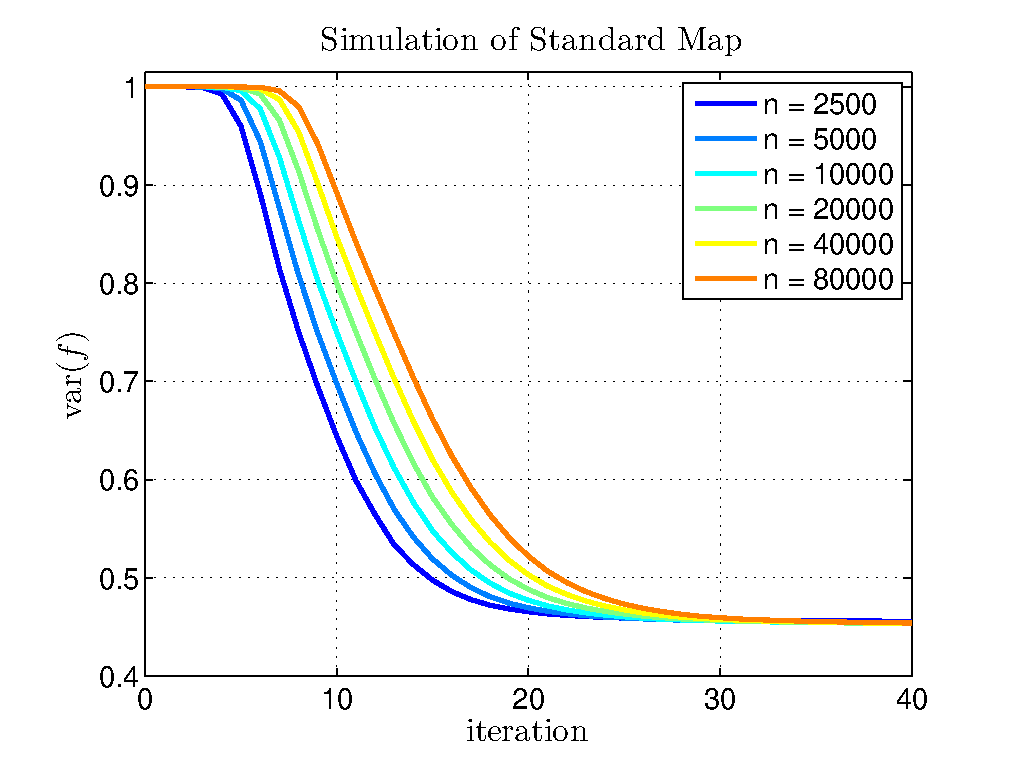
\includegraphics[width=0.55\textwidth,trim=1cm 1cm 0cm 0cm]{standardmapcutoff}&
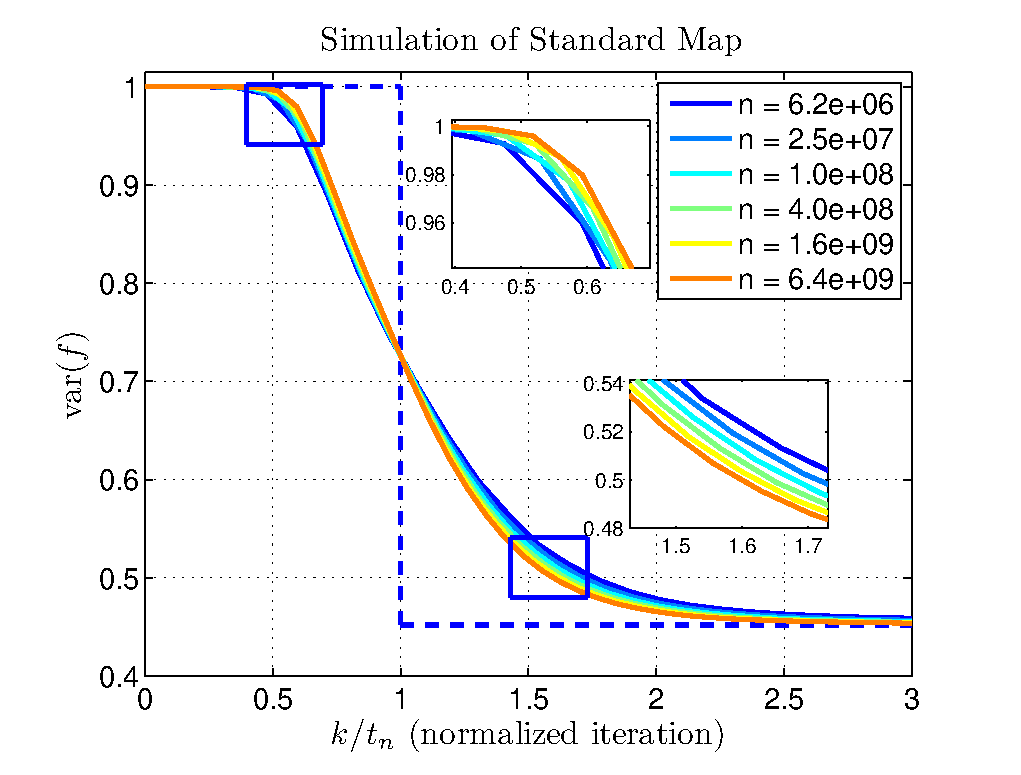
\includegraphics[width=0.55\textwidth,trim=1cm 1cm 0cm 0cm]{standardmapcutoffn}
\end{tabular}
}
\begin{itemize}\setlength{\parskip}{0pt}  \setlength{\itemsep}{5pt} \setlength{\topsep}{0pt}
\item Standard map, $\epsilon = 0.3$, $f^0 = \cos(2\pi x_2)$.
\item $(M,m) = (1,0.4521)$, Cutoff time: $t_n =\min \{ k \mid \text{var}(f^k_n)< \frac{M+m}{2}\} $
\end{itemize}
%%%%%%%%%%%%%%%%%%%%%%%%%%%%%%%%%%%%%%%%%%%%%%%%%%%%%%%%%%%%%%%%%%%%%%%%%
%%%%%%%%%%%%%%%%%%%%%%%%%%%%%%%%%%%%%%%%%%%%%%%%%%%%%%%%%%%%%%%%%%%%%%%%%
%\newpage
%\oursection{Evidence of Standard Map Cutoff}
%%%%%%%%%%%%%%%%%%%%%%%%%%%%%%%%%%%%%%%%%%%%%%%%%%%%%%%%%%%%%%%%%%%%%%%%%
%\centerline{
%\begin{tabular}{rl}%\setlength{\tabcolsep}{-30mm}
%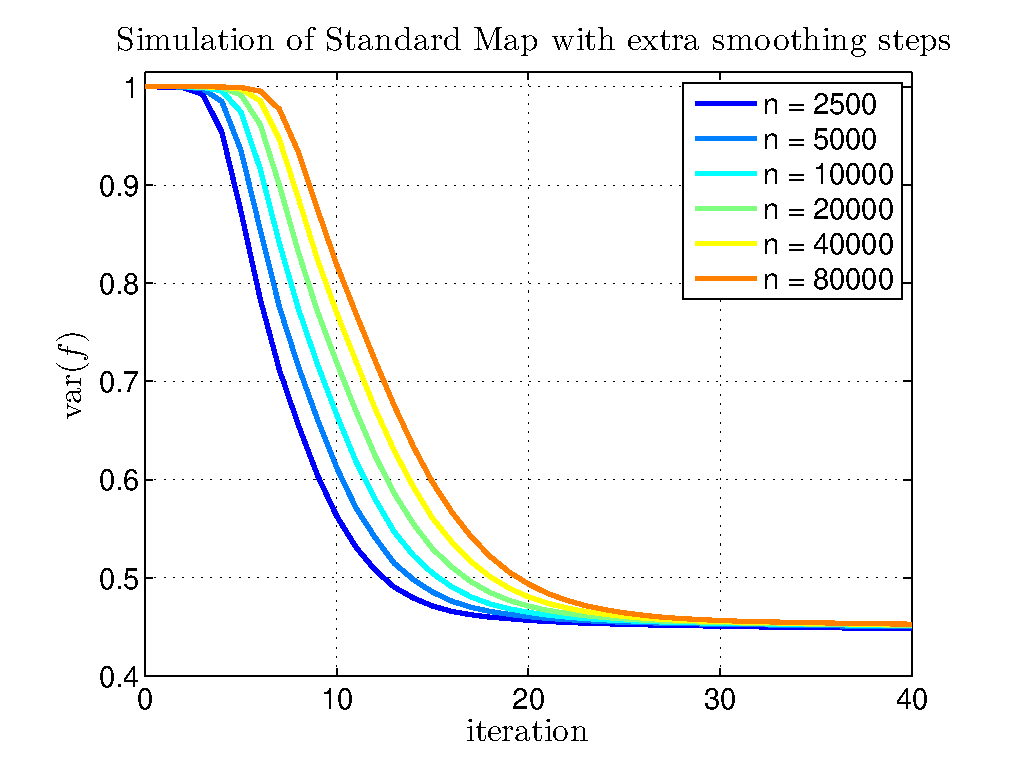
\includegraphics[width=0.55\textwidth,trim=1cm 1cm 0cm 0cm]{standardmapcutoffwithsmoothing}&
%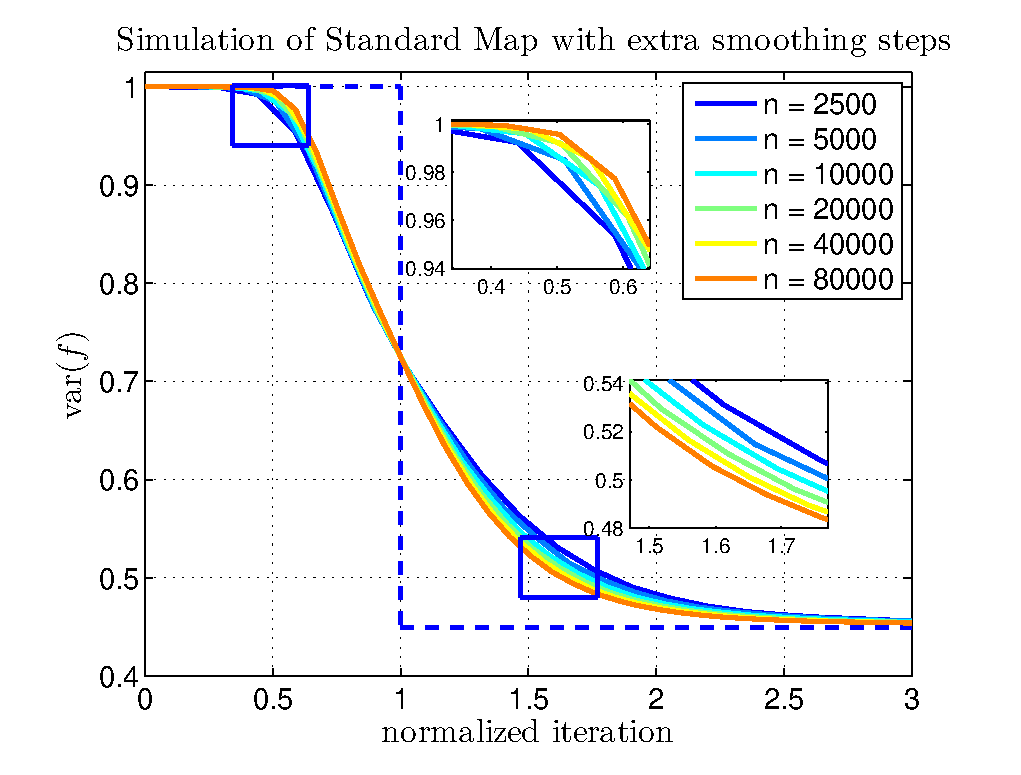
\includegraphics[width=0.55\textwidth,trim=1cm 1cm 0cm 0cm]{standardmapcutoffwithsmoothingn}
%\end{tabular}
%}

%\begin{itemize}\setlength{\parskip}{0pt}  \setlength{\itemsep}{5pt} \setlength{\topsep}{0pt}
%\item Standard map, $\epsilon = 0.3$, $f^0 = \cos(2\pi x_2)$, with additional smoothing steps after each iteration.
%\item $(M,m) = (1,0.4498)$, Cutoff time: $t_n =\min \{ k \mid \text{var}(f^k_n)< \frac{M+m}{2}\} $
%\end{itemize}

%%%%%%%%%%%%%%%%%%%%%%%%%%%%%%%%%%%%%%%%%%%%%%%%%%%%%%%%%%%%%%%%%%%%%%%%%
%%%%%%%%%%%%%%%%%%%%%%%%%%%%%%%%%%%%%%%%%%%%%%%%%%%%%%%%%%%%%%%%%%%%%%%%%
\newpage
\oursection{Evidence of Standard Map Cutoff}
%%%%%%%%%%%%%%%%%%%%%%%%%%%%%%%%%%%%%%%%%%%%%%%%%%%%%%%%%%%%%%%%%%%%%%%%%
\centerline{
\begin{tabular}{rl}%\setlength{\tabcolsep}{-30mm}
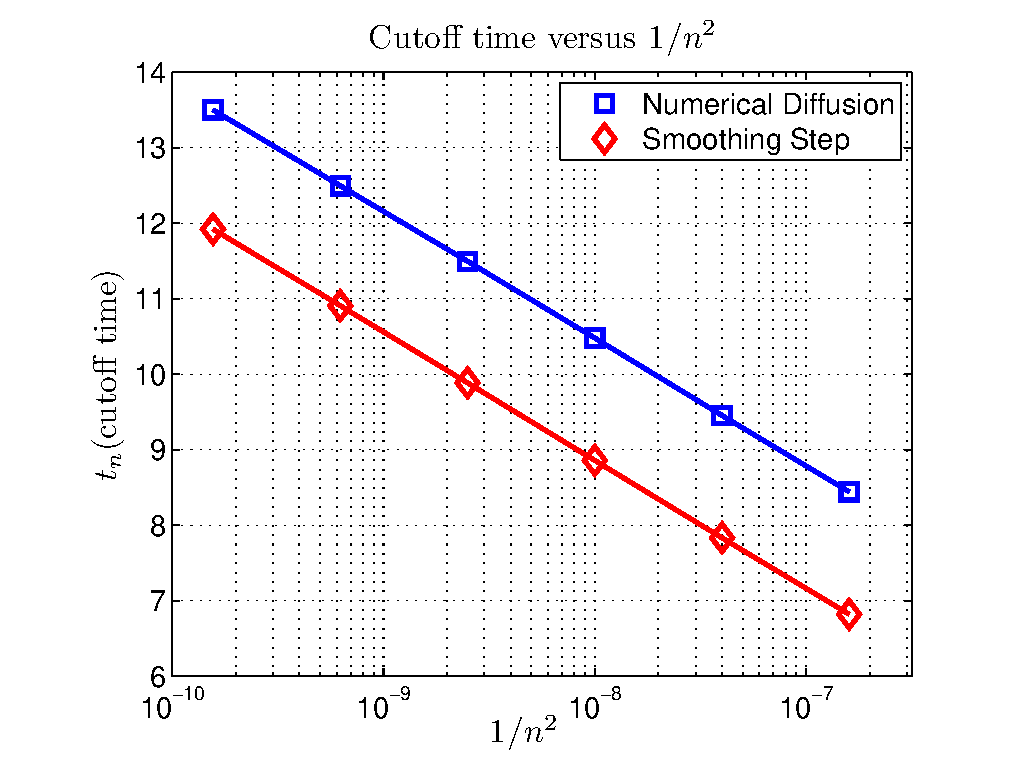
\includegraphics[width=11cm,trim=1cm 1cm 0cm 0cm]{cutofftimevsD}&
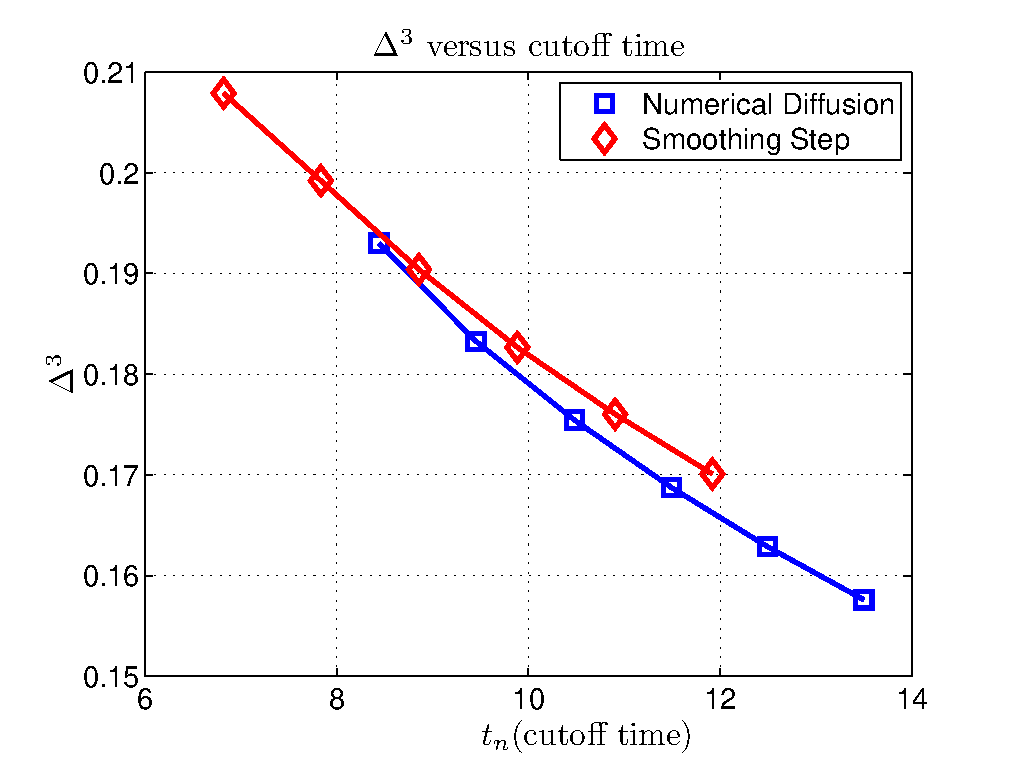
\includegraphics[width=11cm,trim=1cm 1cm 0cm 0cm]{areavscutofftime}
\end{tabular}
}
  \begin{itemize}
  \item Measure distance to sharp transition:
    \begin{equation*}
      c^{\infty}(x) = \begin{cases}
        M, &\text{if } x < 1, \\
        m, &\text{otherwise}
      \end{cases}
      \qquad
      \Delta^l = \int_0^l | c^k(x)-c^{\infty}(x)|\,dx
    \end{equation*}
  \end{itemize}
  
%%%%%%%%%%%%%%%%%%%%%%%%%%%%%%%%%%%%%%%%%%%%%%%%%%%%%%%%%%%%%%%%%%%%%%%%%
\newpage
\oursection{More about Standard Map Cutoff}
%%%%%%%%%%%%%%%%%%%%%%%%%%%%%%%%%%%%%%%%%%%%%%%%%%%%%%%%%%%%%%%%%%%%%%%%%
%%%%%%%%%%%%%%%%%%%%%%%%%%%%%%%%%%%%%%%%%%%%%%%%%%%%%%%%%%%%%%%%%%%%%%%%%
\begin{itemize}
  \item It's really a cutoff.
  \item Only looks slow because we can't simulate large systems($64\times 10^8$ states already).    
  \item Is this the right frame?
    \begin{itemize}
      \item Frequency domain approaches.
      \item How do people study finite Markov Chain cutoffs?($2^{1000} \approx 10^{301}$) An exact model reduction. 
      \item Symbolic Dynamics. 
    \end{itemize}
\end{itemize}


%%%%%%%%%%%%%%%%%%%%%%%%%%%%%%%%%%%%%%%%%%%%%%%%%%%%%%%%%%%%%%%%%%%%%%%%%
%%%%%%%%%%%%%%%%%%%%%%%%%%%%%%%%%%%%%%%%%%%%%%%%%%%%%%%%%%%%%%%%%%%%%%%%%
%%%%%%%%%%%%%                 TOPIC c                          %%%%%%%%%%
%%%%%%%%%%%%%%%%%%%%%%%%%%%%%%%%%%%%%%%%%%%%%%%%%%%%%%%%%%%%%%%%%%%%%%%%%
%%%%%%%%%%%%%%%%%%%%%%%%%%%%%%%%%%%%%%%%%%%%%%%%%%%%%%%%%%%%%%%%%%%%%%%%%


\newpage
\oursection{\mytopicc}
   \begin{itemize}
      \item Tent Map ``Cutoff''
      \item Cutoff Phenomenon of Random Walks on Finite Groups
      \item Symbolic Dynamics and Stochastic Symbol sequence
      \item Create Cutoffs 
   \end{itemize}

%%%%%%%%%%%%%%%%%%%%%%%%%%%%%%%%%%%%%%%%%%%%%%%%%%%%%%%%%%%%%%%%%%%%%%%%%
%%%%%%%%%%%%%%%%%%%%%%%%%%%%%%%%%%%%%%%%%%%%%%%%%%%%%%%%%%%%%%%%%%%%%%%%%
\newpage
\oursection{Tent Map ``Cutoff''}
%%%%%%%%%%%%%%%%%%%%%%%%%%%%%%%%%%%%%%%%%%%%%%%%%%%%%%%%%%%%%%%%%%%%%%%%%
%\begin{example} %\textbf{Tent Map}
%\begin{figure}
\centerline{
\begin{tabular}{rcl}
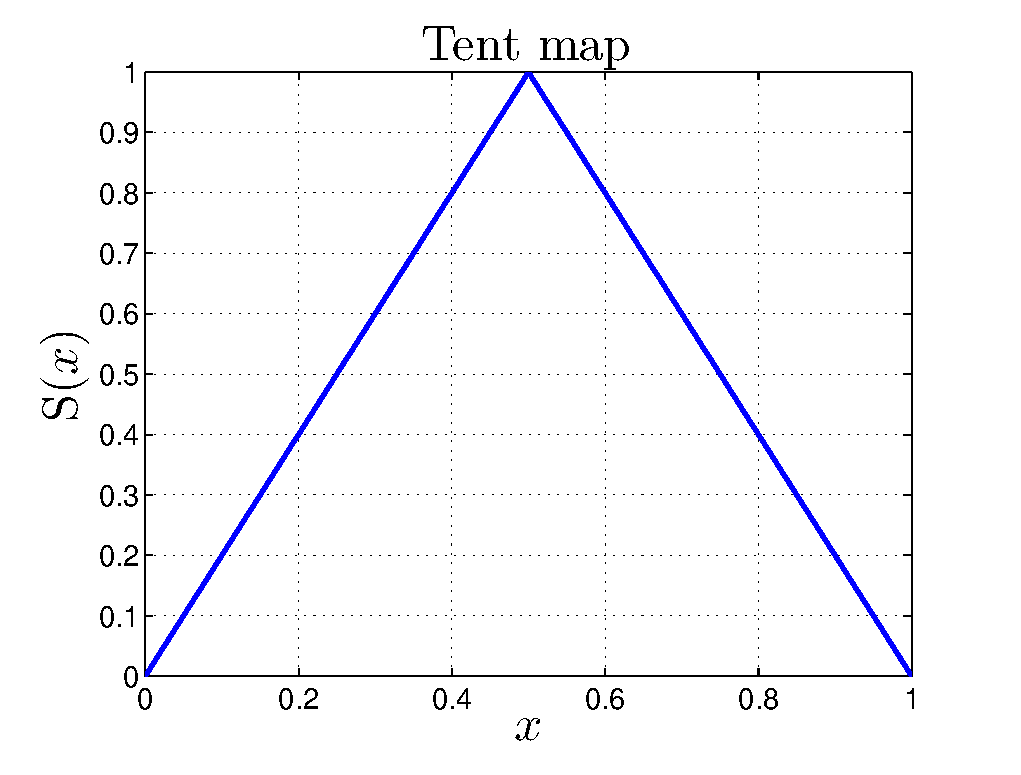
\includegraphics[width=0.34\textwidth,trim=1cm 1cm 1cm 1cm]{tentmap}&
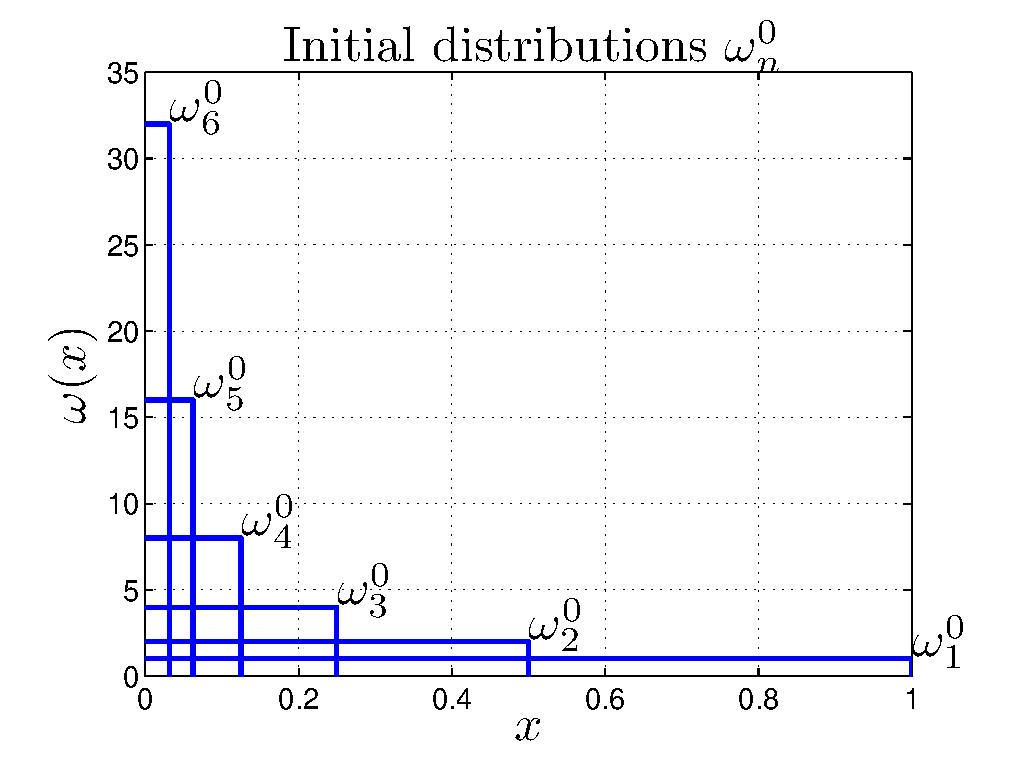
\includegraphics[width=0.34\textwidth,trim=1cm 1cm 1cm 1cm]{tentmapomega0}&
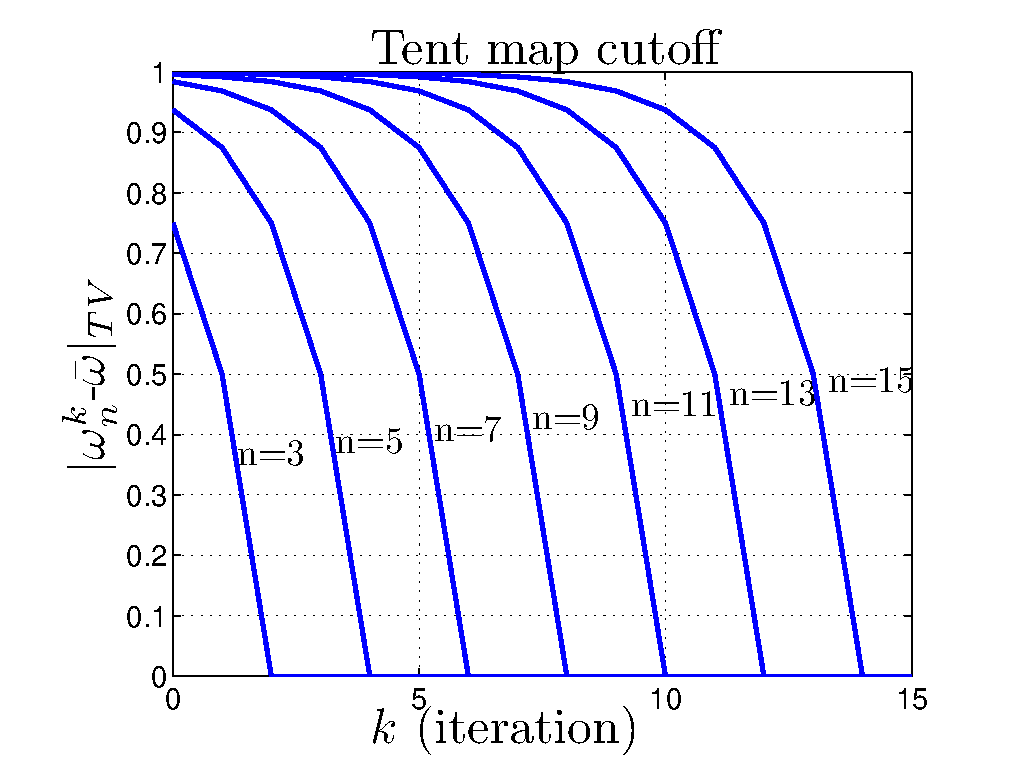
\includegraphics[width=0.34\textwidth,trim=1cm 1cm 1cm 1cm]{tentmapcutoff}
\end{tabular}
}
%\end{figure}
\vspace{-1cm}
   \begin{eqnarray}
   \label{tentmap}
     x \leftarrow S_\text{tent}(x) \equiv 1-2\left|x-\frac{1}{2}\right|,\,\,\,
     P_S(\omega_n^k(x)) = \frac{1}{2}\left(\omega_n^k\left(\frac{x}{2}\right)+\omega_n^k\left(1-\frac{x}{2}\right) \right)\nonumber
   \\[-1.4cm] \nonumber
   \end{eqnarray}
with the following initial distributions on $[0 ,1]$,
  \begin{eqnarray}
  \label{tentmapinitial}
  \\[-1.8cm] \nonumber
    \omega_n^0 = \left\{ \begin{tabular}{c}
                      $\frac{1}{\mu_n}$, \mbox{  if  } $x \le \mu_n$\\
                      $0$, \mbox{  otherwise}
                      \end{tabular}\right.
  \\[-1.6cm] \nonumber
  \end{eqnarray}
where $\mu_1 = 1$, and $\mu_{n+1} = \frac{\mu_n}{2}$.

%\end{example}
%%%%%%%%%%%%%%%%%%%%%%%%%%%%%%%%%%%%%%%%%%%%%%%%%%%%%%%%%%%%%%%%%%%%%%%%%
%%%%%%%%%%%%%%%%%%%%%%%%%%%%%%%%%%%%%%%%%%%%%%%%%%%%%%%%%%%%%%%%%%%%%%%%%
\newpage
\oursection{Revisit random walk on an $n$-dimensional hypercube}
%%%%%%%%%%%%%%%%%%%%%%%%%%%%%%%%%%%%%%%%%%%%%%%%%%%%%%%%%%%%%%%%%%%%%%%%%

%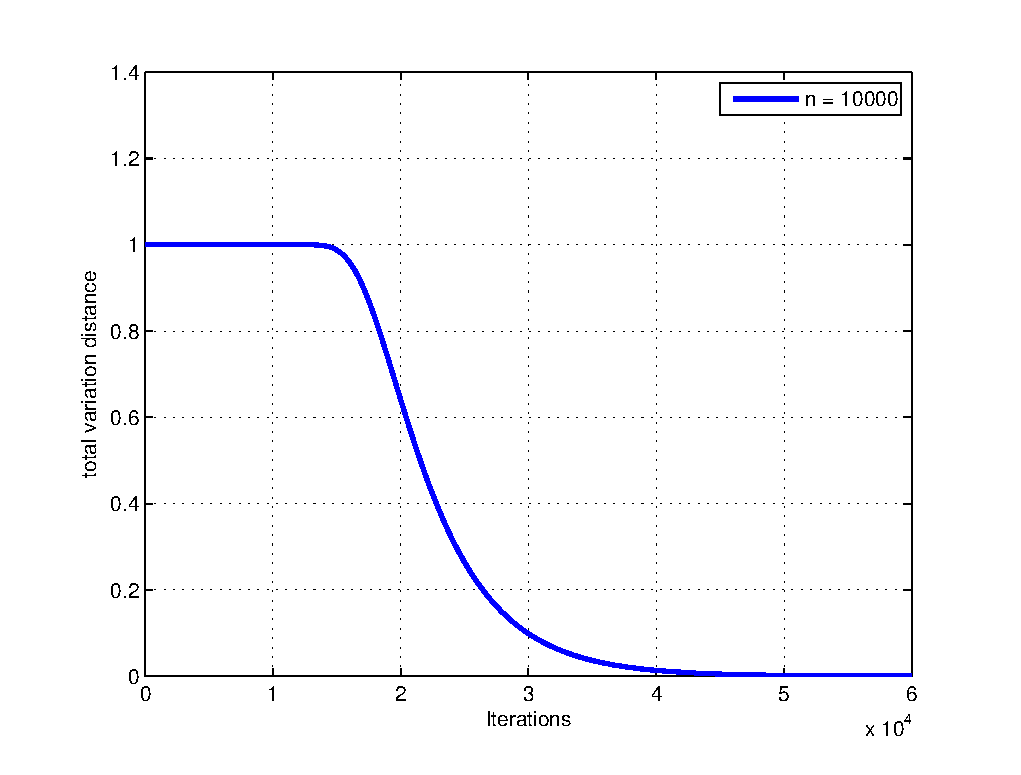
\includegraphics[width=0.45\textwidth,trim=1cm -1cm 0cm 0cm]{cutoffexample}
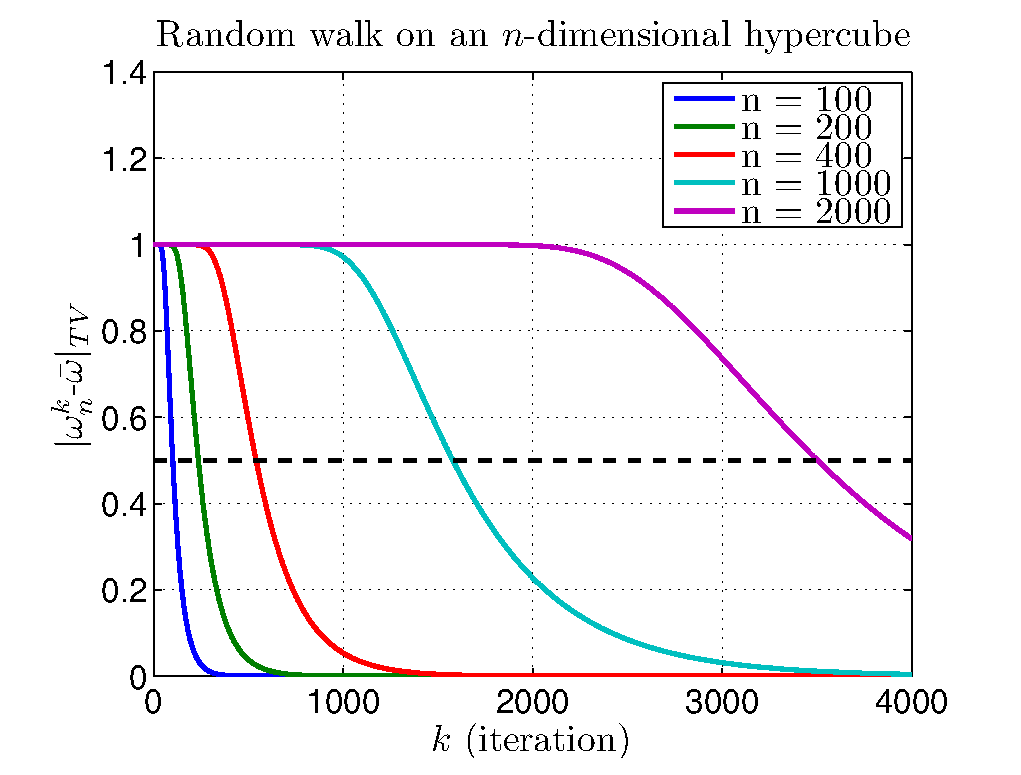
\includegraphics[width=0.45\textwidth,trim=1cm -1cm 0cm 0cm]{rdwalk}
\parbox[b]{12cm}{
  (Diaconis 1990)Let $k = \frac{1}{4}n\log{n}+cn$. Then for fixed $c \in \{-\infty,\infty\}$, as $n \rightarrow \infty$,
\begin{eqnarray}
\label{rdwalkshape}
 |\omega^k_n - \bar{\omega} |_{TV} \sim \erf\left(\frac{e^{-2c}}{\sqrt{8}}\right)
\end{eqnarray}
   }
\begin{itemize}
\item The shape of the cutoff is called ``normal shape''.
\end{itemize}


%%%%%%%%%%%%%%%%%%%%%%%%%%%%%%%%%%%%%%%%%%%%%%%%%%%%%%%%%%%%%%%%%%%%%%%%%
%%%%%%%%%%%%%%%%%%%%%%%%%%%%%%%%%%%%%%%%%%%%%%%%%%%%%%%%%%%%%%%%%%%%%%%%%
\newpage
\oursection{Our Goal}
%%%%%%%%%%%%%%%%%%%%%%%%%%%%%%%%%%%%%%%%%%%%%%%%%%%%%%%%%%%%%%%%%%%%%%%%%
\begin{itemize}
\item Goal: Generate a sequence of $\omega_n^0$ such that when they are evolved by a chaotic map, $|\omega_n^k-\bar{\omega}|_{TV}$ has the same limiting behavior as one sees in the random walk on an $n$-dimensional hypercube problem.
\end{itemize}
We do:
\begin{itemize}
\item Observe why RW has the ``normal'' cutoff shape.
\item Overcome the problem of evolving $\omega_n^k$ for a set of $\omega_n^0\in\bar{\Omega}$, by extending the symbolic dynamics of chaotic maps.
\item Find the upper and lower bounds of $|\omega_n^k-\bar{\omega}|_{TV}$, which characterize the limiting behavior of it.
\end{itemize}


%%%%%%%%%%%%%%%%%%%%%%%%%%%%%%%%%%%%%%%%%%%%%%%%%%%%%%%%%%%%%%%%%%%%%%%%%
%%%%%%%%%%%%%%%%%%%%%%%%%%%%%%%%%%%%%%%%%%%%%%%%%%%%%%%%%%%%%%%%%%%%%%%%%
\newpage
\oursection{What creates the ``normal shape''?\\ A Model Reduction View}
%%%%%%%%%%%%%%%%%%%%%%%%%%%%%%%%%%%%%%%%%%%%%%%%%%%%%%%%%%%%%%%%%%%%%%%%%

Ehrenfests' Urn Problem
\begin{itemize}%\setlength{\parskip}{0pt}  \setlength{\itemsep}{5pt} \setlength{\topsep}{0pt}
\item Two urns and $n$ balls. To start, all the balls are in urn $1$. Each time, a ball is randomly chosen and moved to the other urn.
\item The state of the Markov chain is the number of balls in urn $1$.
\item The system has $n+1$ states, and $\bar{\omega}(i) = {n \choose i}/2^n$.
\item This problem is equivalent to the random walk on a hypercube problem--as if we put all the states having equal distance to $\mathbf{0}$ together to becomes a new state.
\end{itemize}


%%%%%%%%%%%%%%%%%%%%%%%%%%%%%%%%%%%%%%%%%%%%%%%%%%%%%%%%%%%%%%%%%%%%%%%%%
%%%%%%%%%%%%%%%%%%%%%%%%%%%%%%%%%%%%%%%%%%%%%%%%%%%%%%%%%%%%%%%%%%%%%%%%%
\newpage
\oursection{What creates the ``normal'' shape?\\ A Model Reduction View}
%%%%%%%%%%%%%%%%%%%%%%%%%%%%%%%%%%%%%%%%%%%%%%%%%%%%%%%%%%%%%%%%%%%%%%%%%


\centerline{
\scalebox{0.6}[0.6]{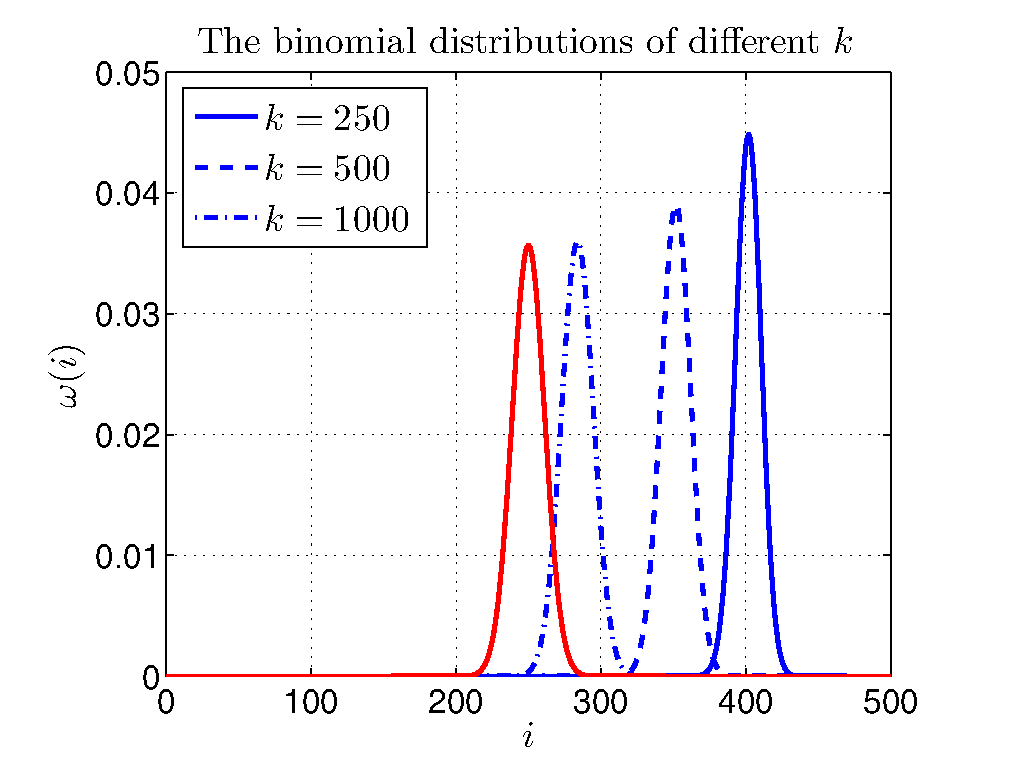
\includegraphics{deltaMexample2a}}
            \scalebox{0.6}[0.6]{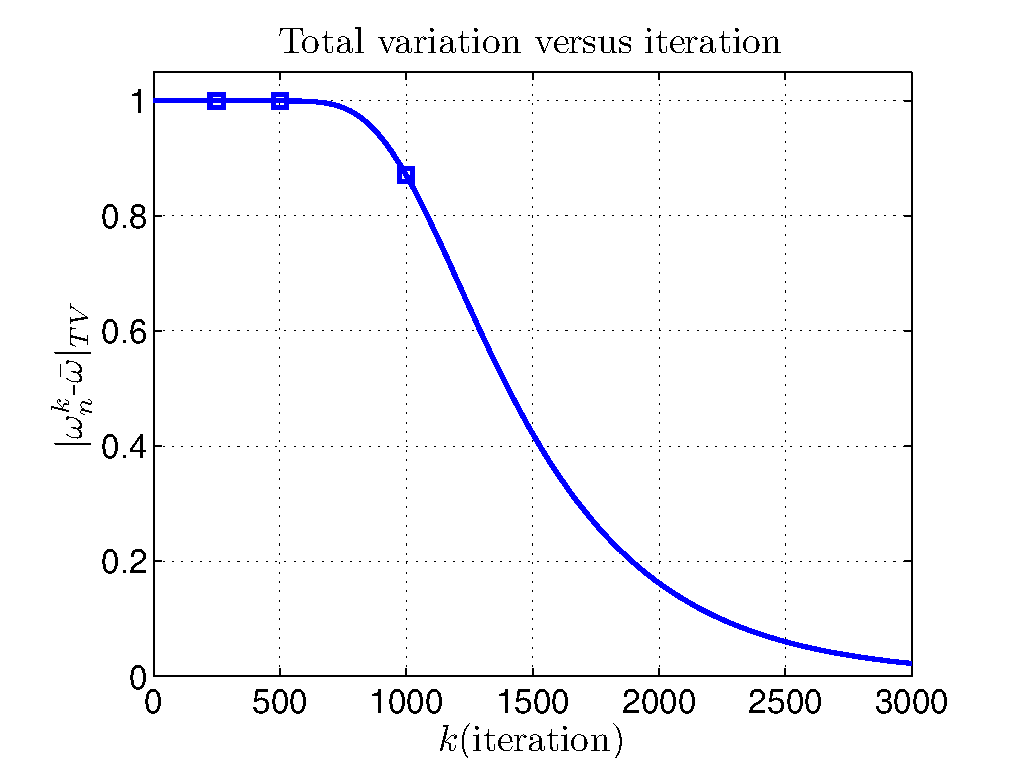
\includegraphics{ehrenfasttv}}
}
\vspace{-1cm}
\begin{itemize}\setlength{\parskip}{0pt}  \setlength{\itemsep}{5pt} \setlength{\topsep}{0pt}
\item The error function comes from the limit of the difference between two binomial distribution.
\item The exponential function comes from the ``moving speed'' of the binomial distribution. 
\end{itemize}
%%%%%%%%%%%%%%%%%%%%%%%%%%%%%%%%%%%%%%%%%%%%%%%%%%%%%%%%%%%%%%%%%%%%%%%%%
%%%%%%%%%%%%%%%%%%%%%%%%%%%%%%%%%%%%%%%%%%%%%%%%%%%%%%%%%%%%%%%%%%%%%%%%%
%\newpage
%\oursection{Symbolic Dynamics(for $1$-D Chaotic Maps) }
%%%%%%%%%%%%%%%%%%%%%%%%%%%%%%%%%%%%%%%%%%%%%%%%%%%%%%%%%%%%%%%%%%%%%%%%%

%\begin{itemize}\setlength{\parskip}{0pt}  \setlength{\itemsep}{5pt} \setlength{\topsep}{0pt}
%     \item Symbol list $\mathcal{S} = \{L,R\}$. Map $S$ has invariant set $\Lambda$, $x\in \Lambda$
%     \item  $s_i \in \mathcal{S}$, $s= \{.s_0s_1\cdots s_n\cdots\} \in \Sigma$
%     \item  $\phi: \Lambda \rightarrow \Sigma$
%     \item $\sigma: \Sigma \rightarrow \Sigma $, shift operator
%           $$\sigma(s)= \{.s_1s_2\cdots s_n\cdots\}$$
%     \item $S(x) = \phi^{-1}\circ \sigma \circ \phi(x)$,
%           \begin{equation*}
%          \xymatrix{
%              \Lambda  \ar[d]_{\phi} \ar[r]^{S}
%              & \Lambda   \ar[d]^{\phi} \\
%          \Sigma \ar[r]_{\sigma}
%              & \Sigma}
%           \end{equation*}
%\end{itemize}

%%%%%%%%%%%%%%%%%%%%%%%%%%%%%%%%%%%%%%%%%%%%%%%%%%%%%%%%%%%%%%%%%%%%%%%%%
%%%%%%%%%%%%%%%%%%%%%%%%%%%%%%%%%%%%%%%%%%%%%%%%%%%%%%%%%%%%%%%%%%%%%%%%%
\newpage
\oursection{Symbolic Dynamics(for $1$-D Chaotic Maps) }
%%%%%%%%%%%%%%%%%%%%%%%%%%%%%%%%%%%%%%%%%%%%%%%%%%%%%%%%%%%%%%%%%%%%%%%%%

\begin{itemize}\setlength{\parskip}{0pt}  \setlength{\itemsep}{5pt} \setlength{\topsep}{0pt}
     \item Symbol list $\mathcal{S} = \{L,R\}$. Map $S$ has invariant set $\Lambda$, $x\in \Lambda$.
     \item  $s_i \in \mathcal{S}$, $s= \{.s_0s_1\cdots s_n\cdots\} \in \Sigma$.
     \item  $\phi: \Lambda \rightarrow \Sigma$.
            \begin{itemize}
            \item Partition invariant set into $\Lambda_L \cup \Lambda_R$.
            \item $s_i \equiv \phi(x)_i =  \begin{cases} 
                           L \text{, if } S^i(x)\in \Lambda_L\\
                           R \text{, if } S^i(x)\in \Lambda_R
                         \end{cases}   $
            \end{itemize} 
     \item $\sigma: \Sigma \rightarrow \Sigma $, shift operator : $\sigma(s)= \{.s_1s_2\cdots s_n\cdots\}$.
     \item $S(x) = \phi^{-1}\circ \sigma \circ \phi(x)$: Chaotic maps $S(x)$ are homeomorphic to the shift map on
        space of symbol sequences.
\end{itemize}
\begin{example}\textbf{Symbolic Dynamics of Tent Map}
\vspace{-0.7cm}
\begin{itemize}\setlength{\parskip}{0pt}  \setlength{\itemsep}{5pt} \setlength{\topsep}{0pt}
     \item $\Lambda_L=[0,0.5]$, $\Lambda_R=(0.5,1]$, $x = 0.3457$, 
           $s = \phi(x) = \{.LRRRLR...\}$, and $\sigma \circ \phi(x) = \{.RRRLR...\}$.
\end{itemize}
\end{example}
%%%%%%%%%%%%%%%%%%%%%%%%%%%%%%%%%%%%%%%%%%%%%%%%%%%%%%%%%%%%%%%%%%%%%%%%%
%%%%%%%%%%%%%%%%%%%%%%%%%%%%%%%%%%%%%%%%%%%%%%%%%%%%%%%%%%%%%%%%%%%%%%%%%
%\newpage
%\oursection{Symbolic Dynamics of Tent Map }
%%%%%%%%%%%%%%%%%%%%%%%%%%%%%%%%%%%%%%%%%%%%%%%%%%%%%%%%%%%%%%%%%%%%%%%%%

%\centerline{
%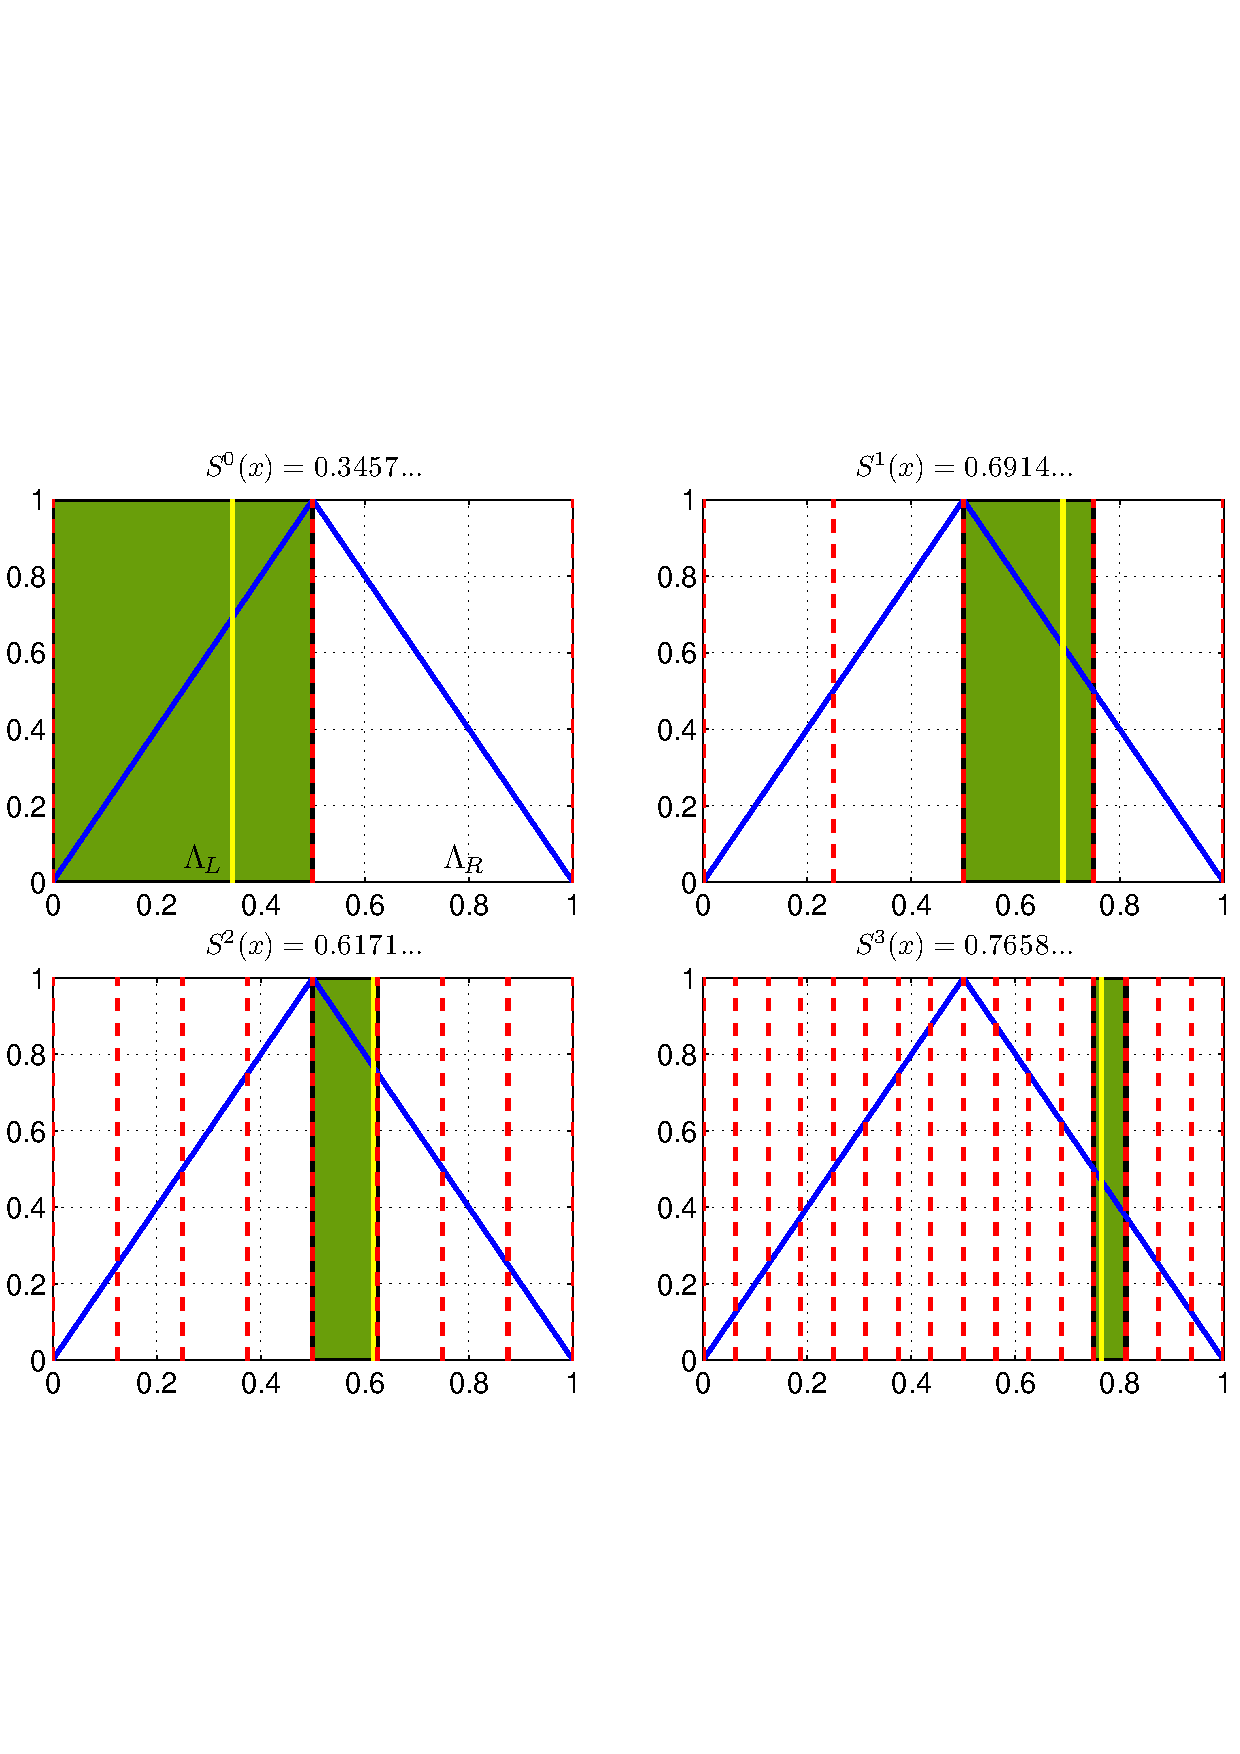
\includegraphics[width=0.7\textwidth]{tentmapplot2}
%}
%$x = 0.3457$, and $ \phi(x)=\{.LRRRLR...\}$.
%%%%%%%%%%%%%%%%%%%%%%%%%%%%%%%%%%%%%%%%%%%%%%%%%%%%%%%%%%%%%%%%%%%%%%%%%
%%%%%%%%%%%%%%%%%%%%%%%%%%%%%%%%%%%%%%%%%%%%%%%%%%%%%%%%%%%%%%%%%%%%%%%%%
\newpage
\oursection{Stochastic Symbol Sequence }
%%%%%%%%%%%%%%%%%%%%%%%%%%%%%%%%%%%%%%%%%%%%%%%%%%%%%%%%%%%%%%%%%%%%%%%%%
\begin{itemize}\setlength{\parskip}{0pt}  \setlength{\itemsep}{5pt} \setlength{\topsep}{0pt}
    \item   $S   \sim $ symbol sequence. 
    \item   $P_S \sim $ stochastic symbol sequence.
\end{itemize}

\begin{definition} \textbf{Stochastic symbol sequence.}
Consider $\mathcal{S}$ to be the symbol list. Let $\Delta$ be the collection of all
semi-infinite sequences of elements in $[0,1]$. We define $\delta^\star \in \Delta$ for each
symbol $\star \in \mathcal{S}$ as
 \begin{align}
 \begin{split}
 \delta^\star &= \{.\delta_0^\star \delta_1^\star\cdots \delta_n^\star\cdots\} \\
 %\delta^R &= \{.\delta_0^R \delta_1^R\cdots \delta_n^R\cdots\}
 \end{split}
 \end{align}
with $\delta^\star_i \in [0,1]$ for all $i$.
\end{definition}
\begin{itemize}\setlength{\parskip}{0pt}  \setlength{\itemsep}{5pt} \setlength{\topsep}{0pt}
  \item $\sigma: \Delta \rightarrow \Delta $, shift operator
    $$\sigma(\delta^L)= \{.\delta^L_1\delta^L_2\cdots
           \delta^L_n\cdots\}$$
\end{itemize}
%%%%%%%%%%%%%%%%%%%%%%%%%%%%%%%%%%%%%%%%%%%%%%%%%%%%%%%%%%%%%%%%%%%%%%%%%
%%%%%%%%%%%%%%%%%%%%%%%%%%%%%%%%%%%%%%%%%%%%%%%%%%%%%%%%%%%%%%%%%%%%%%%%%
\newpage
\oursection{Stochastic Symbol Sequence }
%%%%%%%%%%%%%%%%%%%%%%%%%%%%%%%%%%%%%%%%%%%%%%%%%%%%%%%%%%%%%%%%%%%%%%%%%

\begin{itemize}\setlength{\parskip}{0pt}  \setlength{\itemsep}{5pt} \setlength{\topsep}{0pt}

    \item Consider $\mathcal{S} =\{L,R \}$, $\psi^L :\Omega \rightarrow \Delta$
               \begin{eqnarray*}
               \label{psidef}
               %\delta^L_i = \int_{\Lambda_L} P^i_S \omega(x)dx \text{,   and  }
               \delta^L_i = \int_{\Lambda_L} P^i_S \left(\omega(x)\right)dx \text{, for all }i\ge0
               \\[-1.5cm]
               \end{eqnarray*}
    \item For $x\in \Lambda$ having distribution $\omega$, the interpretation of $\delta_i^L$ is
             \begin{eqnarray*}
             \label{deltaistar}
             \delta_i^L = \prob(\phi(x)_i = L) \text{, for } \text{ for all }i
              \end{eqnarray*}
             (Remember $\phi(x)_i=L$ if $S^i(x)\in \Lambda_L$ for a deterministic $x$.)

    \item If $\mathcal{S} =\{L,R\}$, $\delta^R=1-\delta^L$. (For convenience, $\delta \equiv \delta^L$.)
    \item  Define $\psi \equiv \psi^L$, we have,
           \begin{lemma}
                $$\psi \circ P_S = \sigma \circ \psi$$
           \end{lemma}

\end{itemize}

   %\item  $\mathcal{S} = \{L,R\}$, $\delta_i^{L},\delta_i^{R} \in [0, 1]$,
   %        \begin{eqnarray}
   %        \delta^L = \{\cdots \delta_{-n}^L\cdots \delta_{-1}^L.\delta_0^L \delta_1^L\cdots \delta_n^L\cdots\} \nonumber\\
   %        \delta^R = \{\cdots \delta_{-n}^R\cdots \delta_{-1}^R.\delta_0^R \delta_1^R\cdots \delta_n^R\cdots\} \nonumber
   %        \end{eqnarray}

    %
    %$$\sigma(\delta^L)= \{\cdots \delta^L_{-n}\cdots \delta^L_{-1}\delta^L_0.\delta^L_1\cdots
    %       \delta^L_n\cdots\}$$

%%%%%%%%%%%%%%%%%%%%%%%%%%%%%%%%%%%%%%%%%%%%%%%%%%%%%%%%%%%%%%%%%%%%%%%%%
%%%%%%%%%%%%%%%%%%%%%%%%%%%%%%%%%%%%%%%%%%%%%%%%%%%%%%%%%%%%%%%%%%%%%%%%%
\newpage
\oursection{Stochastic Symbol Sequence }
%%%%%%%%%%%%%%%%%%%%%%%%%%%%%%%%%%%%%%%%%%%%%%%%%%%%%%%%%%%%%%%%%%%%%%%%%
\vspace{-0.7cm}
\begin{itemize}\setlength{\parskip}{0pt}  \setlength{\itemsep}{5pt} \setlength{\topsep}{0pt}
   \item Unfortunately, $\psi$ is not invertible. There are many $\omega\in \Omega$ which maps to the same $\delta$
   \item So we restrict $\omega$ to the following space,
         \vspace{-0.2cm}
        \begin{eqnarray}
        \label{DefOmegabar}
        \bar{\Omega} = \left\{ \omega \left| \omega(x) = \lim_{n \rightarrow \infty} \prod_{i=0}^n \beta^{\phi(x)_i}_i \right. \right\}
        \end{eqnarray}
        where $\beta^L_i \in [0,1]$, $\beta^R_i=1-\beta^L_i$.
   \item Now $\psi:\bar{\Omega} \rightarrow \Delta$ is invertible. For $\omega \in \bar{\Omega}$, $\delta^L_i=\psi(\omega)_i = \beta^L_i$ for all $i$. 

\end{itemize}
\vspace{0.5cm}

    \begin{lemma} For $x$ having pdf $\omega\in \bar{\Omega}$, $s = \phi(x)$, then $s_0,s_1,s_2,...$ are all independent to each other. 
         \end{lemma}


%%%%%%%%%%%%%%%%%%%%%%%%%%%%%%%%%%%%%%%%%%%%%%%%%%%%%%%%%%%%%%%%%%%%%%%%%
%%%%%%%%%%%%%%%%%%%%%%%%%%%%%%%%%%%%%%%%%%%%%%%%%%%%%%%%%%%%%%%%%%%%%%%%%
\newpage
\oursection{Stochastic Symbol Sequence }
%%%%%%%%%%%%%%%%%%%%%%%%%%%%%%%%%%%%%%%%%%%%%%%%%%%%%%%%%%%%%%%%%%%%%%%%%
\begin{itemize}\setlength{\parskip}{0pt}  \setlength{\itemsep}{5pt} \setlength{\topsep}{0pt}

   \item $P_S$ is the Perron-Frobenius operator of $S$
         \begin{eqnarray}
         P_S (\omega) \in \bar{\Omega}, \mbox{if } \omega \in \bar{\Omega} \nonumber
         \end{eqnarray}
   \item More importantly,
         \begin{eqnarray}
         P_S= \psi^{-1}\circ \sigma \circ \psi  \nonumber
         \end{eqnarray}
   \item Reminder: the above procedure is to find the subspace $\bar{\Omega}$ such that when $\omega\in\bar{\Omega}$, we can find $P_S^i(\omega)$ for all $i$ easily.
\end{itemize}
%%%%%%%%%%%%%%%%%%%%%%%%%%%%%%%%%%%%%%%%%%%%%%%%%%%%%%%%%%%%%%%%%%%%%%%%%
%%%%%%%%%%%%%%%%%%%%%%%%%%%%%%%%%%%%%%%%%%%%%%%%%%%%%%%%%%%%%%%%%%%%%%%%%
\newpage
\oursection{Total Variation Distance in $\bar{\Omega}$}
%%%%%%%%%%%%%%%%%%%%%%%%%%%%%%%%%%%%%%%%%%%%%%%%%%%%%%%%%%%%%%%%%%%%%%%%%
\begin{itemize}\setlength{\parskip}{0pt}  \setlength{\itemsep}{5pt} \setlength{\topsep}{0pt}
    \item $\omega$, $\hat{\omega}\in{\bar{\Omega}}$ have stochastic symbol sequences  $\{\delta^L, \delta^R\}$ and $\{\hat{\delta}^L,\hat{\delta}^R \}$, respectively.
          \begin{eqnarray}
            \label{infiniteTV}
            |\omega-\hat{\omega}|_{TV} = \frac{1}{2} \lim_{n \rightarrow \infty}  \sum_{s\in\Sigma} \left|
                                     \prod_{i=0}^n\delta_i^{s_i}-\prod_{i=0}^n\hat{\delta}_i^{s_i}  \right| \nonumber
          \end{eqnarray}
    \item $\delta_i^L = \hat{\delta}_i^L$ when $i\notin \theta$, and $|\theta| = p$.
          \begin{eqnarray}
           \label{finiteTV}
            |\omega-\hat{\omega}|_{TV} = \frac{1}{2} \sum_{s\in\Sigma_p}  \left|
                             \prod_{i\in \theta}\delta_i^{s_i}-\prod_{i\in\theta}\hat{\delta}_i^{s_i}  \right| \nonumber
          \end{eqnarray}
   where $\Sigma_p$ are all $\{L,R\}$ combinations of $p$ symbols($2^p$).
   %\item without loss of generality, assume $\delta^L_i =\delta^R_i$ for all $i$, and let $\delta \equiv \delta^L $
\end{itemize}

%%%%%%%%%%%%%%%%%%%%%%%%%%%%%%%%%%%%%%%%%%%%%%%%%%%%%%%%%%%%%%%%%%%%%%%%%
%%%%%%%%%%%%%%%%%%%%%%%%%%%%%%%%%%%%%%%%%%%%%%%%%%%%%%%%%%%%%%%%%%%%%%%%%
\newpage
\oursection{Total Variation Distance to Invariant Distribution}
%%%%%%%%%%%%%%%%%%%%%%%%%%%%%%%%%%%%%%%%%%%%%%%%%%%%%%%%%%%%%%%%%%%%%%%%%
\begin{itemize}\setlength{\parskip}{0pt}  \setlength{\itemsep}{5pt} \setlength{\topsep}{0pt}
    \item The invariant distribution of map $S$ is $\bar{\omega}$.
          $$\bar{\delta}\equiv \psi(\bar{\omega}) = \left\{.\frac{1}{2}\frac{1}{2}\frac{1}{2}...\right\}  $$
    \item $\omega \mapsto |\omega-\bar{\omega}|_{TV}$ is convex, so  $\delta \mapsto |\psi^{-1}(\delta)-\bar{\omega}|_{TV} $ is also convex.
    \item Using convexity, we can prove
          \begin{lemma}
          \label{alldifflemma}
           $\delta$ and $\hat{\delta}$ are two stochastic symbol sequences, each corresponds to the probability distribution $\omega$ and $\hat{\omega}$, respectively. Suppose there exists a bijection $\beta: i \mapsto j$ such that $|\delta_i-\frac{1}{2}| \ge |\hat{\delta}_j-\frac{1}{2} |$ for all $i\in \mathbb{Z}$, then
          \begin{eqnarray}
          |\omega-\bar{\omega} |_{TV} \ge|\hat{\omega}-\bar{\omega} |_{TV}
          \end{eqnarray}
\end{lemma}
\end{itemize}
%%%%%%%%%%%%%%%%%%%%%%%%%%%%%%%%%%%%%%%%%%%%%%%%%%%%%%%%%%%%%%%%%%%%%%%%%
%%%%%%%%%%%%%%%%%%%%%%%%%%%%%%%%%%%%%%%%%%%%%%%%%%%%%%%%%%%%%%%%%%%%%%%%%
\newpage
\oursection{Evaluate the Total Variation Distance}
%%%%%%%%%%%%%%%%%%%%%%%%%%%%%%%%%%%%%%%%%%%%%%%%%%%%%%%%%%%%%%%%%%%%%%%%%
\begin{itemize}\setlength{\parskip}{0pt}  \setlength{\itemsep}{0pt} \setlength{\topsep}{0pt}
\vspace{-1cm}
    \item Consider the flolowing two sequences
        \begin{eqnarray}
        \\[-1.5cm] \nonumber
         \hat{\delta} 
               = \{.\underbrace{\hat{\delta}_{\star} \hat{\delta}_{\star} \cdots \hat{\delta}_{\star}}_{p}\frac{1}{2}\frac{1}{2}\cdots\},  
         \bar{\delta}= \left\{.\frac{1}{2}\frac{1}{2}\frac{1}{2}\cdots\right\}\nonumber
        \\[-1.5cm] \nonumber
        \end{eqnarray}         
        %   $\hat{\delta}_0 =\hat{\delta}_1= \cdots = \hat{\delta}_{p-1}$
   \item The TV can be evaluated by finding the difference between two binomial distributions. %$|\psi^{-1}(\delta)-\psi^{-1}(\bar{\delta)}|^{TV}$
        \begin{eqnarray}
           |\hat{\omega}-\bar{\omega}|_{TV}
                     & = &\frac{1}{2} \sum_{s\in\Sigma_p}
                           \left| \prod_{i\in \theta}\hat{\delta}_i^{s_i}-\prod_{i\in\theta}\bar{\delta}_i^{s_i}  \right| \nonumber \\
                     & = &\frac{1}{2}  \sum_{k=0}^p {p \choose k}
                           \left|(\hat{\delta}_\star)^k (1-\hat{\delta}_\star)^{p-k} - \frac{1}{2^p} \right| \nonumber\\
                     & = &\frac{1}{2} \sum_{k=0}^p\left|\text{binomial}(k;p,\hat{\delta}_\star)-\text{binomial}\left(k;p,\frac{1}{2}\right)\right| \nonumber
     %                & \rightarrow &\erf \left( \sqrt{\frac{p}{2}}\left((\delta_{\star}^m)-\frac{1}{2}\right)\right) \text{, when } p\rightarrow \infty \text{, and } \delta_{\star}^m \rightarrow \frac{1}{2}
                    % & = &\frac{1}{2}  \sum_{k=0}^p \left|{p \choose k}
                    %       (\delta_\star)^k (1-\delta_\star)^{p-k} -{p \choose k} \frac{1}{2^p} \right|\nonumber
        \end{eqnarray}
\end{itemize}
%%%%%%%%%%%%%%%%%%%%%%%%%%%%%%%%%%%%%%%%%%%%%%%%%%%%%%%%%%%%%%%%%%%%%%%%%
%%%%%%%%%%%%%%%%%%%%%%%%%%%%%%%%%%%%%%%%%%%%%%%%%%%%%%%%%%%%%%%%%%%%%%%%%
\newpage
\oursection{Upper Bound and Lower Bound}
%%%%%%%%%%%%%%%%%%%%%%%%%%%%%%%%%%%%%%%%%%%%%%%%%%%%%%%%%%%%%%%%%%%%%%%%%
% the plot of ub,lb theorems
\begin{theorem}\textbf{Lower Bound.}
\label{theoremlb}
$\delta$ and $\bar{\delta}$ are two stochastic symbol sequences, each corresponds to the probability distribution $\omega$ and the invariant distribution $\bar{\omega}$, respectively. Suppose there is a set $\theta \subset \mathbb{Z}^++\{0\} $, $|\theta|=p$ such that for all $i \in \theta$, $|\delta_i-\frac{1}{2}|>\epsilon$, then
\begin{eqnarray}
\label{lbineq}
|\omega-\bar{\omega}|_{TV} \ge \mathbf{I}_{\frac{1}{2}}(p-k^*,k^*+1) - \mathbf{I}_{\frac{1}{2}-\epsilon}(p-k^*,k^*+1)
\end{eqnarray}
with
\begin{eqnarray}
\label{kstar}
k^* =  \left\lfloor p \frac{\log{2}+\log{(\frac{1}{2}-\epsilon)} }{\log{(\frac{1}{2}-\epsilon)}-\log{(\frac{1}{2}+\epsilon})} \right\rfloor
\end{eqnarray}
where $\mathbf{I}$ is the regularized incomplete beta function.
\end{theorem}
In this theorem, we bound $|\omega-\bar{\omega}|_{TV}$ by choosing $\hat{\delta}_\star = \frac{1}{2}+\epsilon$. 
%%%%%%%%%%%%%%%%%%%%%%%%%%%%%%%%%%%%%%%%%%%%%%%%%%%%%%%%%%%%%%%%%%%%%%%%%
%%%%%%%%%%%%%%%%%%%%%%%%%%%%%%%%%%%%%%%%%%%%%%%%%%%%%%%%%%%%%%%%%%%%%%%%%
%\newpage
%\oursection{The Limit of the Bounds}
%%%%%%%%%%%%%%%%%%%%%%%%%%%%%%%%%%%%%%%%%%%%%%%%%%%%%%%%%%%%%%%%%%%%%%%%%
%\begin{itemize}
%   \item
%         \begin{align*}
%         \hat{\delta}      = \{.\underbrace{\hat{\delta}_\star \hat{\delta}_\star \cdots \hat{\delta}_\star}_{p}\frac{1}{2}\frac{1}{2}\cdots\}, \,\,\,
%         \bar{\delta}  = \left\{.\frac{1}{2}\frac{1}{2}\frac{1}{2}\cdots\right\}
%         \end{align*}
%\end{itemize}
%\begin{theorem}
%\label{theoremapproxlb} $\bar{\omega}$ and $\hat{\omega}$ are two probability distributions, and have the stochastic
%symbol sequences $\bar{\delta}$ and $\delta$ as defined above, respectively. Let $p
%\rightarrow \infty$ and $\hat{\delta}_{\star} \rightarrow \frac{1}{2}$, then one has
%\begin{align}
%\begin{split}
%  \label{lbublimit}
%                 |\hat{\omega}-\bar{\omega}|_{TV}
%               & =  \erf \left( \sqrt{\frac{p}{2}}\left((\hat{\delta}_{\star})-\frac{1}{2}\right)\right)
%\end{split}
%\end{align}


%\end{theorem}


%%%%%%%%%%%%%%%%%%%%%%%%%%%%%%%%%%%%%%%%%%%%%%%%%%%%%%%%%%%%%%%%%%%%%%%%%
%%%%%%%%%%%%%%%%%%%%%%%%%%%%%%%%%%%%%%%%%%%%%%%%%%%%%%%%%%%%%%%%%%%%%%%%%
%\newpage
%\oursection{Moving and Reshaping}
%%%%%%%%%%%%%%%%%%%%%%%%%%%%%%%%%%%%%%%%%%%%%%%%%%%%%%%%%%%%%%%%%%%%%%%%%
%\centerline{
%\begin{tabular}{cc}
%\scalebox{1.1}[1.1]{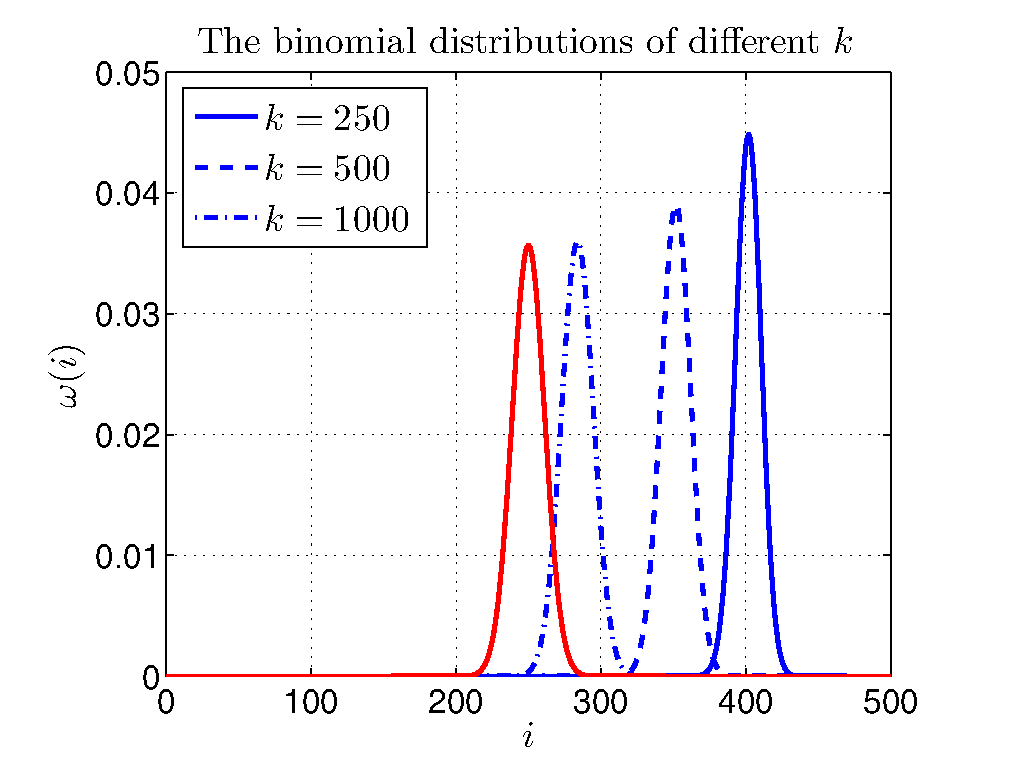
\includegraphics[width=0.38\textwidth,trim=0cm 0cm 0cm 0cm]{deltaMexample2a}}
%\scalebox{1.1}[1.1]{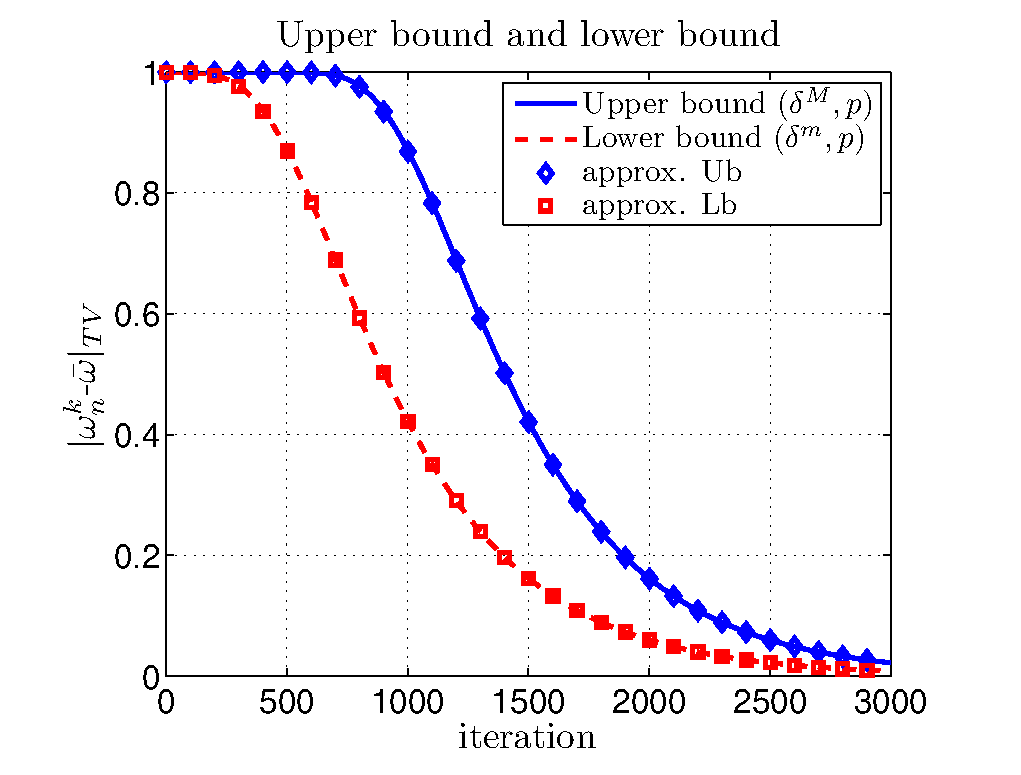
\includegraphics[width=0.38\textwidth,trim=0cm 0cm 0cm 0cm]{deltaMexample2b}} %\\
%\end{tabular}
%}
%\centerline{
%\scalebox{1.1}[1.1]{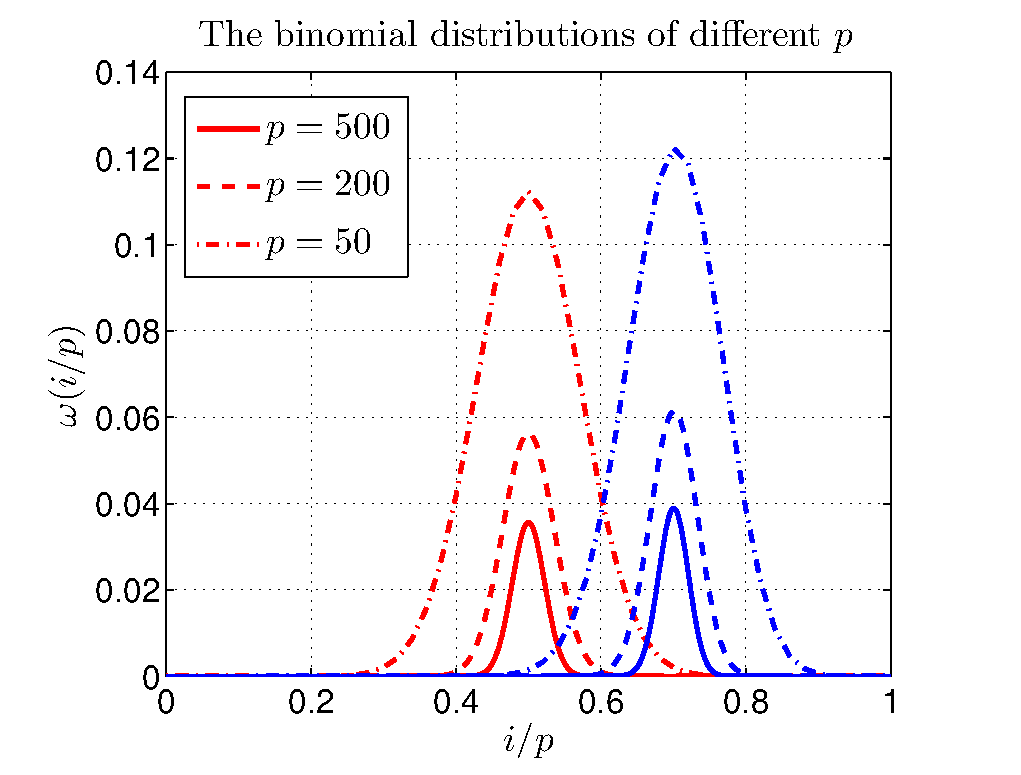
\includegraphics[width=0.38\textwidth,trim=0cm 0cm 0cm 0cm]{deltaMexample1a}}
%\scalebox{1.1}[1.1]{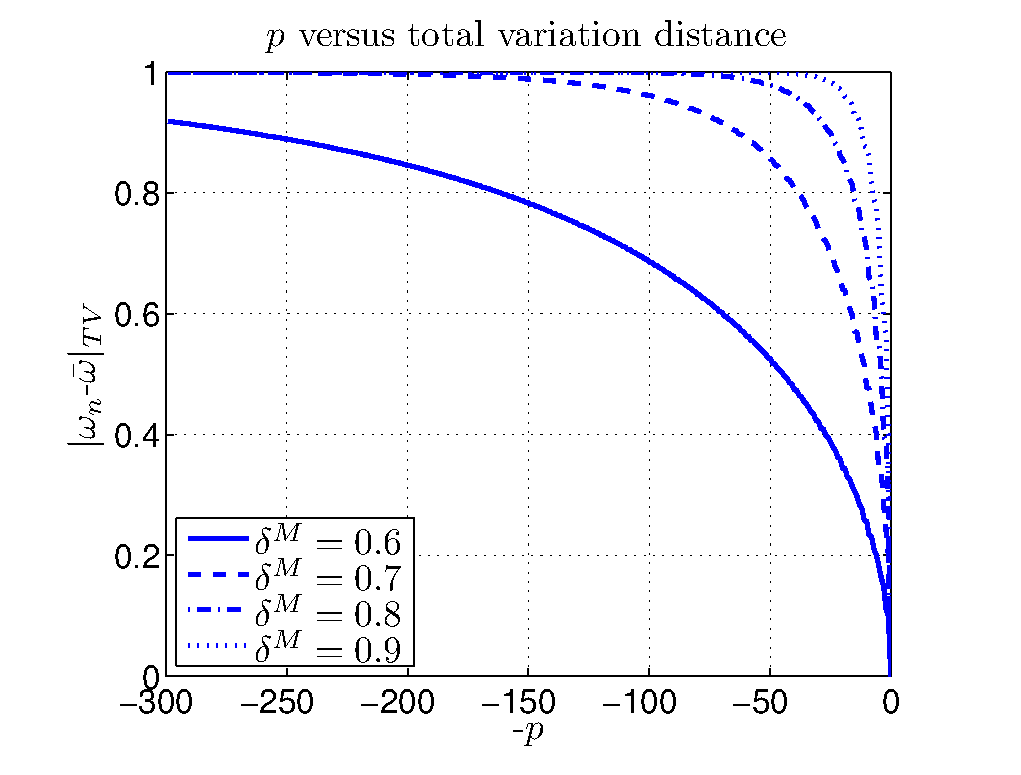
\includegraphics[width=0.38\textwidth,trim=0cm 0cm 0cm 0cm]{deltaMexample1b}}
%}
%%%%%%%%%%%%%%%%%%%%%%%%%%%%%%%%%%%%%%%%%%%%%%%%%%%%%%%%%%%%%%%%%%%%%%%%%
%%%%%%%%%%%%%%%%%%%%%%%%%%%%%%%%%%%%%%%%%%%%%%%%%%%%%%%%%%%%%%%%%%%%%%%%%
\newpage
\oursection{Create Cutoffs}
%%%%%%%%%%%%%%%%%%%%%%%%%%%%%%%%%%%%%%%%%%%%%%%%%%%%%%%%%%%%%%%%%%%%%%%%%
\begin{theorem}
Let $\omega_n^0 \in \bar{\Omega}$ has stochastic symbol sequence as the following,

\vspace{-1cm}

 \begin{eqnarray}
    \psi(\omega^0_n) =  \{.(\delta_n)_0 (\delta_n)_1 (\delta_n)_2 \cdots\}
 \end{eqnarray}
where $(\delta_n)_i = \min\{\frac{1}{2}+\epsilon_n r_n^i,1\}$, and
 \begin{align}
 %\begin{split}
   \epsilon_n = \sqrt{\frac{n(1-r_n)}{4}}, \,\,\,\,
            r_n = e^{-\frac{2}{n}}
 %\end{split}
 \end{align}
The family $(\Omega,\bar{\omega},(\omega^k_n)_{k=0,1,...})_{n=1,2,...}$ presents a Total Variation-cutoff. In fact,
Let $k = \frac{1}{4}n\log{n}+cn $, then for fixed $c\in \{-\infty,\infty\}$. as $n\rightarrow \infty$,
\begin{eqnarray}
\label{erfbound}
 %|\omega^k_n - \bar{\omega} |_{TV} \sim \erf \left(\frac{e^{-2c}}{\sqrt{8}}\right)
          \erf \left(\frac{e^{-2c-1}}{\sqrt{8}}\right)\le  |\omega^k_n - \bar{\omega} |_{TV} \le \erf \left(\frac{e^{-2c}}{\sqrt{8}}\right)
\end{eqnarray}
\end{theorem}

%%%%%%%%%%%%%%%%%%%%%%%%%%%%%%%%%%%%%%%%%%%%%%%%%%%%%%%%%%%%%%%%%%%%%%%%%
%%%%%%%%%%%%%%%%%%%%%%%%%%%%%%%%%%%%%%%%%%%%%%%%%%%%%%%%%%%%%%%%%%%%%%%%%
\newpage
\oursection{The Implication}
%%%%%%%%%%%%%%%%%%%%%%%%%%%%%%%%%%%%%%%%%%%%%%%%%%%%%%%%%%%%%%%%%%%%%%%%%
\begin{itemize}%\setlength{\parskip}{0pt}  \setlength{\itemsep}{5pt} \setlength{\topsep}{0pt}
\item We show that it is possible to generate a sequence of $\omega_n^0$ such that when they are evolved by any $1$-D chaotic map with symbolic dynamics, they present the desired cutoff.
\item We can create any cutoff with normal shape by the same way. 
\item Having symbolic dynamics is sufficient to produce cutoff. 
\end{itemize}
%%%%%%%%%%%%%%%%%%%%%%%%%%%%%%%%%%%%%%%%%%%%%%%%%%%%%%%%%%%%%%%%%%%%%%%%%
%%%%%%%%%%%%%%%%%%%%%%%%%%%%%%%%%%%%%%%%%%%%%%%%%%%%%%%%%%%%%%%%%%%%%%%%%
\newpage
\oursection{Conclusion: What Creates (Chaotic Map) Cutoffs?}
\begin{itemize}
\item ``Almost'' independency. 
\item In the random walk on an hypercube problem, the initial state can be represented as,
\begin{equation*}
    x_n^0 = (0,0,0,0,0,0,0,...) 
\end{equation*}
Each of the coordinate equals $0$ with probability $1$. When $k$ is large the probabilities converge to $\frac{1}{2}$ almost independently.  
\item The symbolic dynamics provides the platform of independency.  

%\item "To people studying finite Markov chains, the fact theorem 3.1 can be proved at all appears like a miracle." - Laurent Saloff-Coste, Probability on Discrete Structures.
\end{itemize}

%%%%%%%%%%%%%%%%%%%%%%%%%%%%%%%%%%%%%%%%%%%%%%%%%%%%%%%%%%%%%%%%%%%%%%%%%%
\end{document}
